
\chapter{Definitions}

\label{app:definitions}

- \textbf{Fully-cooperative settings}: refer to scenarios in which all participants or agents involved are aligned towards achieving a common goal. In these settings, the success of the collective effort is prioritized over individual gains, and the participants work together seamlessly, sharing resources, information, and strategies to maximize the overall outcome.

% - \textbf{Semi-cooperative settings}: refer to scenarios where participants or agents share a partial alignment towards common goals but retain some level of individual objectives or competition.

% - \textbf{Coverage}: refers to the geographic area on the Earth's surface that a satellite can observe, monitor, or communicate with at any given time.


- \textbf{Environment}: An environment is a physical or virtual world whose state
evolves over time and is influenced by the actions of the agents that exist
within the environment. The environment specifies the actions that agents
can take at any point in time, as well as the observations that individual
agents receive about the state of the environment. The states of the environment may be defined as discrete or continuous quantities, or a combination
of both.

-\textbf{Agents}: An agent is an entity which receives information about the state of the
environment and can choose different actions in order to influence the state.
Agents may have different prior knowledge about the environment, such as
the possible states that the environment can be in and how states are affected
by the actions of the agents. Importantly, agents are goal-directed in the
sense that agents have specified goals and choose their actions in order to
achieve their goals.

- \textbf{Policy}: refers to a function used by the agent to select actions (or assign probabilities to selecting each action) given the current state of the environment. If the environment is only partially observed
by the agent, then the policy may be conditioned on the current and past
observations of the agent.

- \textbf{MARL:} a multi-agent system consists of an environment and multiple decision-making
agents that interact in the environment to achieve certain goals.

- \textbf{Finite Markov decision process}: A finite Markov decision process
(MDP) consists of: 
\begin{itemize}
    \item Finite set of states S, with subset of terminal states $\Bar{S} \subset S$
    \item  Finite set of actions A
    \item Reward function R : $S × A × S \rightarrow R$
    \item State transition probability function $T : S × A × S \rightarrow [0, 1]$ such that:
    \begin{equation}
    \forall s \in S, a \in A: \sum_{s' \in S} T(s,a,s') = 1
\end{equation}
    \item Initial state distribution $\mu : S \rightarrow [0, 1]$ such that:
\begin{equation}
    \sum _{s \in S} \mu (s) = 1\  \text{and} \ \forall s \in \Bar{S}: \mu (s) =0 \end{equation}
\end{itemize}


% - \textbf{Event-Triggered Mechanism:} Coordination and control of agents based on specific events or changes in the system's state (like the \textbf{local event detection}: change in state (battery, robotics..), detection of byzantine agents or \textbf{threshold-based triggering}: based on distance or reputation of agents).

% - \textbf{Formation Control: }Coordination and Control of a group of autonomous agents to achieve and maintain a desired geometric configuration. It can be centralized (a central controller guides the entire formation) or decentralized (each entity makes decisions based on local observations).

% - \textbf{Leader Tracking:} Capability of a system to monitor and follow the movements or actions of a designated dynamic leader.


- \textbf{Stochastic Model: } a mathematical approach that incorporates random variables to predict a range of possible outcomes rather than a single deterministic result. It accounts for inherent uncertainties and variability in the system being modeled.


- \textbf{Deterministic Model: }a mathematical approach that predicts a single, specific outcome given a set of initial conditions. It assumes no randomness in the system, so the results are entirely determined by the input parameters.




- \textbf{Greedy policies}: A policy is greedy with respect to a value function it is optimal according to that value function for a one-step problem.



    
\newpage
\chapter{Extended Background}
\label{app:extended_background}
\section{The Multi-Agent Transformer (MAT)}
\label{sec:MAT}

 is a novel encoder-decoder architecture designed to treat cooperative multi-agent reinforcement learning (MARL) as a sequence modeling problem. The core idea is to map a sequence of agent observations $(o_{i_1}, \dots, o_{i_n})$ to a sequence of optimal actions $(a_{i_1}, \dots, a_{i_n})$.

\textbf{Overall Architecture: } As illustrated in  Figure~\ref{fig:mat_architecture}, the MAT architecture is structured as an encoder-decoder model. This design is not arbitrary; it's a direct implementation of the \textbf{Multi-Agent Advantage Decomposition Theorem}. This theorem is the cornerstone of the entire approach, stating that the advantage of a joint action can be decomposed into a sum of local, ordered advantages:
\begin{equation}
    \label{eq:mat_advantage_decomp}
    A_{\pi_{i_{1:n}}}(o, a_{i_{1:n}}) = \sum_{m=1}^{n} A_{\pi_{i_m}}(o, a_{i_{1:m-1}}, a_{i_m})
\end{equation}
This decomposition transforms the complex joint policy optimization into a sequential decision-making process, where each agent's decision is conditioned on the actions of its predecessors in a given permutation. The MAT architecture is designed to explicitly model this sequential dependency.

\textbf{Encoder: Multi-Agent Observation Encoding: } The first stage, the Multi-Agent Observation Encoding block shown in the top half of the diagram, serves as the encoder. Its primary function is to process the joint observations and learn expressive latent representations $(\hat{o}_{i_1}, \dots, \hat{o}_{i_n})$ that capture the complex interrelationships between agents. It uses standard Transformer blocks composed of self-attention and MLPs to achieve this.

Crucially, during training, the encoder is also optimized to learn the agents' value functions. This is accomplished by minimizing the empirical Bellman error via the following loss function:
\begin{equation}
    \label{eq:mat_encoder_loss}
    L_{\text{Encoder}}(\phi) = \frac{1}{Tn} \sum_{m=1}^{n} \sum_{t=0}^{T-1} \left[ R(o_t, a_t) + \gamma V_{\phi'}(\hat{o}_{t+1}^{i_m}) - V_{\phi}(\hat{o}_{t}^{i_m}) \right]^2
\end{equation}
Here, $V_{\phi}$ is the value function parameterized by the encoder's weights $\phi$, and $\phi'$ represents the parameters of a frozen target network, a standard technique for stabilizing training.

\textbf{Decoder: Auto-regressive Action Decoding:} The second stage is the Auto-regressive Action Decoding block, which generates an optimal action for each agent sequentially. This directly implements the sequential dependency from the decomposition theorem. As shown in the bottom half of the diagram, the decoder receives the latent observation representations from the encoder and the sequence of previously generated actions.

Its auto-regressive nature means the policy for agent $i_m$ is conditioned on the latent joint observation and the actions of preceding agents: $\pi_{\theta_{i_m}}(a_{i_m} | \hat{o}_{i_{1:n}}, a_{i_{1:m-1}})$. This is enforced by a masked self-attention mechanism, which ensures that the computation for agent $i_m$ can only attend to the outputs of agents $i_1, \dots, i_{m-1}$.

To train the decoder parameters $\theta$, MAT uses a clipping objective from Proximal Policy Optimization (PPO):
\begin{equation}
    \label{eq:mat_decoder_loss}
    L_{\text{Decoder}}(\theta) = -\frac{1}{Tn} \sum_{m=1}^{n} \sum_{t=0}^{T-1} \min \left( r_t^{i_m}(\theta)\hat{A}_t, \text{clip}(r_t^{i_m}(\theta), 1 \pm \epsilon)\hat{A}_t \right)
\end{equation}
The policy ratio is $r_t^{i_m}(\theta) = \frac{\pi_{\theta_{i_m}}(a_{t}^{i_m} | \hat{o}_{t}^{i_{1:n}}, a_{t}^{i_{1:m-1}})}{\pi_{\theta_{\text{old}}}(a_{t}^{i_m} | \hat{o}_{t}^{i_{1:n}}, a_{t}^{i_{1:m-1}})}$, and $\hat{A}_t$ is an estimate of the joint advantage function, calculated using Generalized Advantage Estimation (GAE) with the value function from the encoder as a baseline.

This design provides a monotonic improvement guarantee while also being highly computationally efficient, as it allows for parallel computation of losses during training (since actions are known from the replay buffer). During inference, actions are generated one by one, as shown by the red dashed feedback loop in the diagram.

\begin{figure}[H]
  \centering
 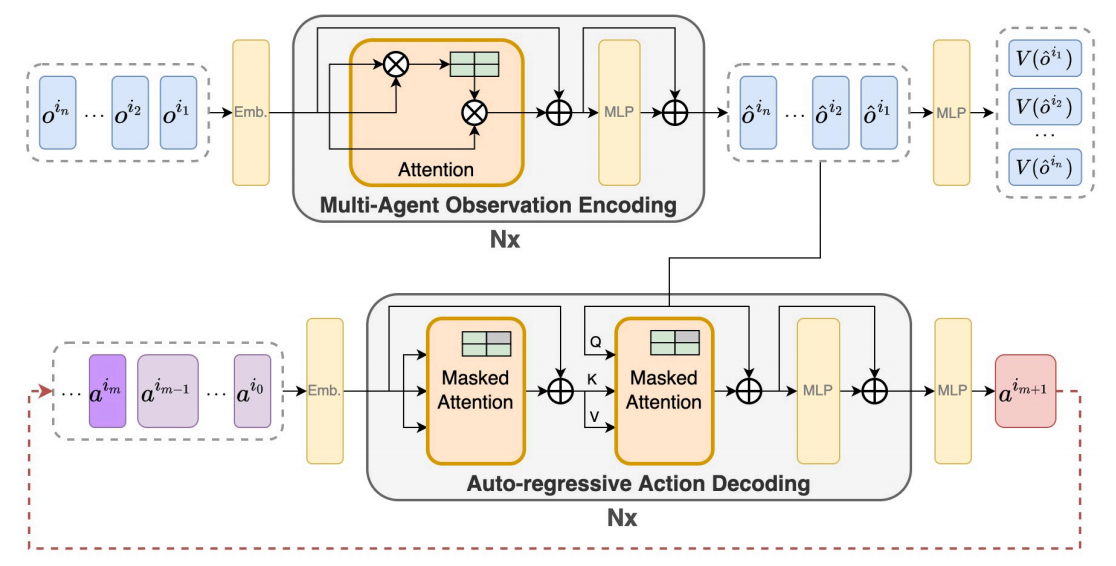
\includegraphics[width=0.75\textwidth]{img_pfe/MAT_arch.PNG}
  \caption{The encoder-decoder architecture of MAT. At each time step, the encoder takes in a sequence of
agents’ observations and encodes them into a sequence of latent representations, which is then passed into
the decoder. The decoder generate each agent’s optimal action in a sequential and auto-regressive manner.
The masked attention blocks ensures agents can only access its preceding agents’ actions during training. (adapted from \parencite{MAT} )}
\label{fig:mat_architecture}
\end{figure}
\FloatBarrier

\section{The Multi-Agent Decision Transformer (MADT)}
\label{sec:MADT}
  Is a novel approach designed to leverage large, offline datasets to pre-train a single, generalizable policy for multi-agent reinforcement learning (MARL) tasks. The core idea is to first treat MARL as a sequence modeling problem for offline pre-training and then fine-tune this model in an online environment to improve performance and sample efficiency. The entire pipeline, as illustrated in the paper's Figure~\ref{fig:madt_architecture}, consists of these two main phases: offline pre-training on static data followed by online fine-tuning through active interaction. The ultimate goal is to create a universal policy that can generalize across different scenarios and tasks with strong few-shot and zero-shot capabilities.

In the offline phase, detailed on the left side of the provided diagram, MADT casts the problem as a conditional sequence modeling task using a Causal Transformer to autoregressively predict an agent's actions based on past events. The learning process uses trajectories where each step is a token $x_t$ composed of the global state, local observation, and action, $x_t = (s_t, o_t^i, a_t^i)$. Notably, this formulation omits the \textit{reward-to-go} signal, as ablation studies found it harmful to online performance. To ensure predictions at timestep $t$ only depend on past inputs, the architecture uses a lower triangular mask $M$ in its attention mechanism, calculated as:
\begin{equation}
\label{eq:madt_att}
    \text{Attention}(Q,K,V) = \text{softmax}\left(\frac{QK^T}{\sqrt{d_k}} + M\right)V
\end{equation}
This offline model is trained with a supervised Cross-Entropy (CE) loss, $L_{\text{CE}}(\theta) = \frac{1}{C} \sum P(a_t) \log P(\hat{a}_t|\tau_t, \hat{a}_{<t}; \theta)$, to imitate the behavior in the dataset.

Since this imitation learning lacks the incentive to maximize rewards, the model then transitions to an online fine-tuning stage. In this phase, as shown on the right side of the diagram, the pre-trained Causal Transformer serves as a shared backbone for separate Actor and Critic networks within a Proximal Policy Optimization (PPO) framework. The Actor network's parameters $\theta_i$ are updated by maximizing the PPO clip objective:
\begin{equation*}
    \theta_i \leftarrow \arg\max_{\theta_i} \mathbb{E}\left[\min\left(w_t(\theta_i) A(s,a_i), \text{clip}(w_t(\theta_i), 1-\epsilon, 1+\epsilon)A(s, a_i)\right)\right]
\end{equation*}
where $w$ is the importance sampling weight. The Critic network's parameters $\phi$ are updated by minimizing the Mean Squared Error (MSE) loss:
\begin{equation}
 \label{eq:madt_loss}
    L_{\phi} = \frac{1}{2} \left( \sum_t \gamma^t r_t - V_{\phi}(s) \right)^2
\end{equation}
% This two-stage process allows MADT to learn a strong prior and then rapidly adapt to maximize rewards, boosting sample efficiency. To ensure the model can generalize across scenarios, it employs several key techniques:
% \begin{itemize}
%     \item Parameter sharing across agents with a one-hot agent ID.
%     \item Feature encoding by padding features to a universal size.
%     \item Action masking to handle different action spaces.
%     \item Reward scaling to balance learning across tasks.
% \end{itemize}
This two-stage process boosts sample efficiency and enables generalization across scenarios through key techniques like parameter sharing, feature padding, action masking, and reward scaling.
\begin{figure}[H]
  \centering
 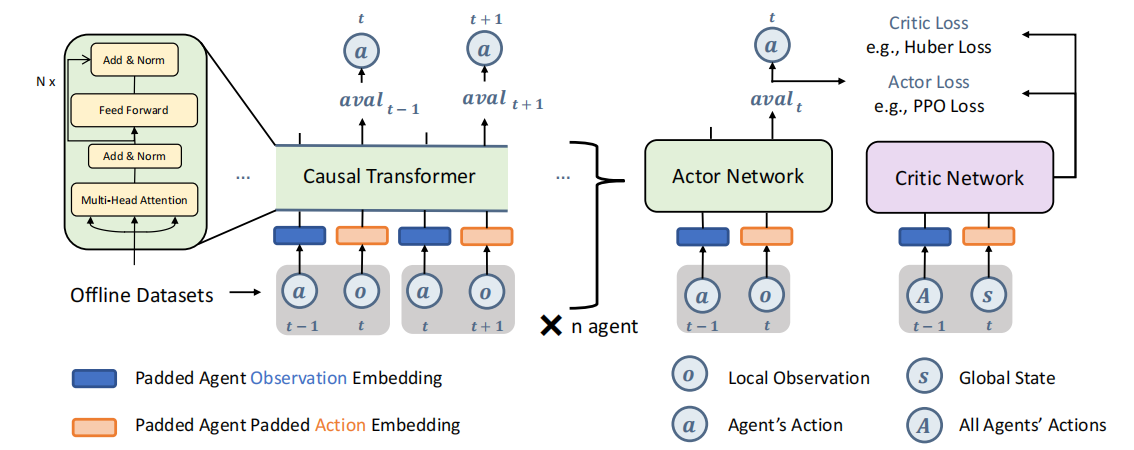
\includegraphics[width=0.75\textwidth]{img_pfe/MADT_arch.PNG}
  \caption{The detailed model structure for offline and online MADT (adapted from \parencite{MADT})}
\label{fig:madt_architecture}
\end{figure}

\section{Formalism of Common Knowledge}
\label{sec:mackrl_details}
\textbf{Common Knowledge in Multi-Agent Systems: } Common knowledge of a group of agents ${\mathcal{G}}$ refers to facts that all members know, and that each individual knows that all other individuals know it, each individual knows that all other individuals know that all the individuals know it, and so on. Any data $\xi$ that are known to all agents before execution/training, like a shared random seed, are obviously common knowledge. Crucially, every agent $a \in {\mathcal{G}}$ can deduce the same history of common knowledge $\tau_t^{\mathcal{G}}$ from its own history $\tau_t^a$ and the commonly known data $\xi$, that is, $\tau_t^{\mathcal{G}} := I_{\mathcal{G}}(\tau_t^a, \xi) = I_{\mathcal{G}}(\tau_t^{\bar{a}}, \xi)$, for all $a, \bar{a} \in {\mathcal{G}}$.

Furthermore, any actions taken by a policy $\pi_{\mathcal{G}}(u_{\text{env}}^{\mathcal{G}} | \tau_t^{\mathcal{G}})$ over the group’s joint action space $U_{\text{env}}^{\mathcal{G}}$ are themselves common knowledge, if the policy is deterministic or pseudo-random with a shared random seed and conditions only on the common history $\tau_t^{\mathcal{G}}$. Common knowledge of subgroups ${\mathcal{G}}_0 \subset \mathcal{G}$ cannot decrease, that is, $I_{{\mathcal{G}}_0}(\tau_t^a, \xi) \supseteq I_{\mathcal{G}}(\tau_t^a, \xi)$.

\textbf{Common Knowledge with Uncertainty:} Given a Dec-POMDP with noisy observations, agents in a group $\mathcal{G}$ might not be able to establish true common knowledge even if sensor noise properties are commonly known \parencite{knowledge_common_knowledge_distributed_env}. Instead, each agent $a$ can only deduce its own beliefs $\tilde{I}_a^{\mathcal{G}}(\tilde{\tau}_t^a)$ over what is commonly known within $\mathcal{G}$, where $\tilde{\tau}_t^a$ is the agent’s belief over what constitutes the groups’ common history. Each agent $a$ can then evaluate its own belief over the group policy $\tilde{\pi}_a^{\mathcal{G}}(u_{\text{env}}^{\mathcal{G}} | \tilde{\tau}_t^{\mathcal{G}})$. In order to minimize the probability of disagreement during decentralized group action selection, agents in $\mathcal{G}$ can perform optimal correlated sampling based on a shared random seed.

\textbf{Learning under common knowledge (LuCK):} is a  cooperative multi-agent reinforcement learning setting, where a Dec-POMDP is augmented by a common knowledge function $I_{\mathcal{G}}$ (or probabilistic common knowledge function $\tilde{I}_a^{\mathcal{G}}$). Groups of agents ${\mathcal{G}}$ can coordinate by learning policies that condition on their common knowledge. In this paper $I_{\mathcal{G}}$ (or $\tilde{I}_a^{\mathcal{G}}$) is fixed a priori, but it could also be learnt during training. The setting accommodates a wide range of real-world and simulated multi-agent tasks. Whenever a task is cooperative and learning is centralised, then agents can naturally learn suitable $I_{\mathcal{G}}$ or $\tilde{I}_a^{\mathcal{G}}$. Policy parameters can be exchanged during training as well and thus become part of the commonly known data $\xi$. Joint policies where coordinated decisions of a group ${\mathcal{G}}$ only condition on the common knowledge of ${\mathcal{G}}$ can be executed in a fully decentralised fashion.

\textbf{Field-of-View Common Knowledge:} is a form of complete-history common knowledge \parencite{knowledge_common_knowledge_distributed_env}, that arises within a Dec-POMDP if agents can deduce parts of other agents’ observations from their own. In this case, an agent group’s common knowledge is the intersection of observations that all members can reconstruct from each other. under some assumptions, common knowledge is the intersection of all agents’ sets of visible objects, if and only if all agents can see each other. This naturally occurs in many interesting real-world tasks, such as autonomous driving and robo-soccer \parencite{robot_soccer}.
\newpage
% \chapter{Analysis of Learning Stability}
% \section{Analysis of Mean Absolute TD-error metric}
% \label{app:td_error_abs_analysis}

% This appendix provides a direct analysis of the learning process by visualizing the mean absolute TD-error. This metric offers insight into the stability and convergence of the agents' underlying value functions. A lower, more stable TD-error indicates that the agents are making more accurate predictions and have learned a more reliable policy. The following plots compare our LI-MA2E framework against the baseline Random Masking across the tested SMAC scenarios.

% %-------------------------------------------------
% \subsection{Scenario: \texttt{3m}}
% %-------------------------------------------------

% \begin{figure}[H]
%     \centering
%     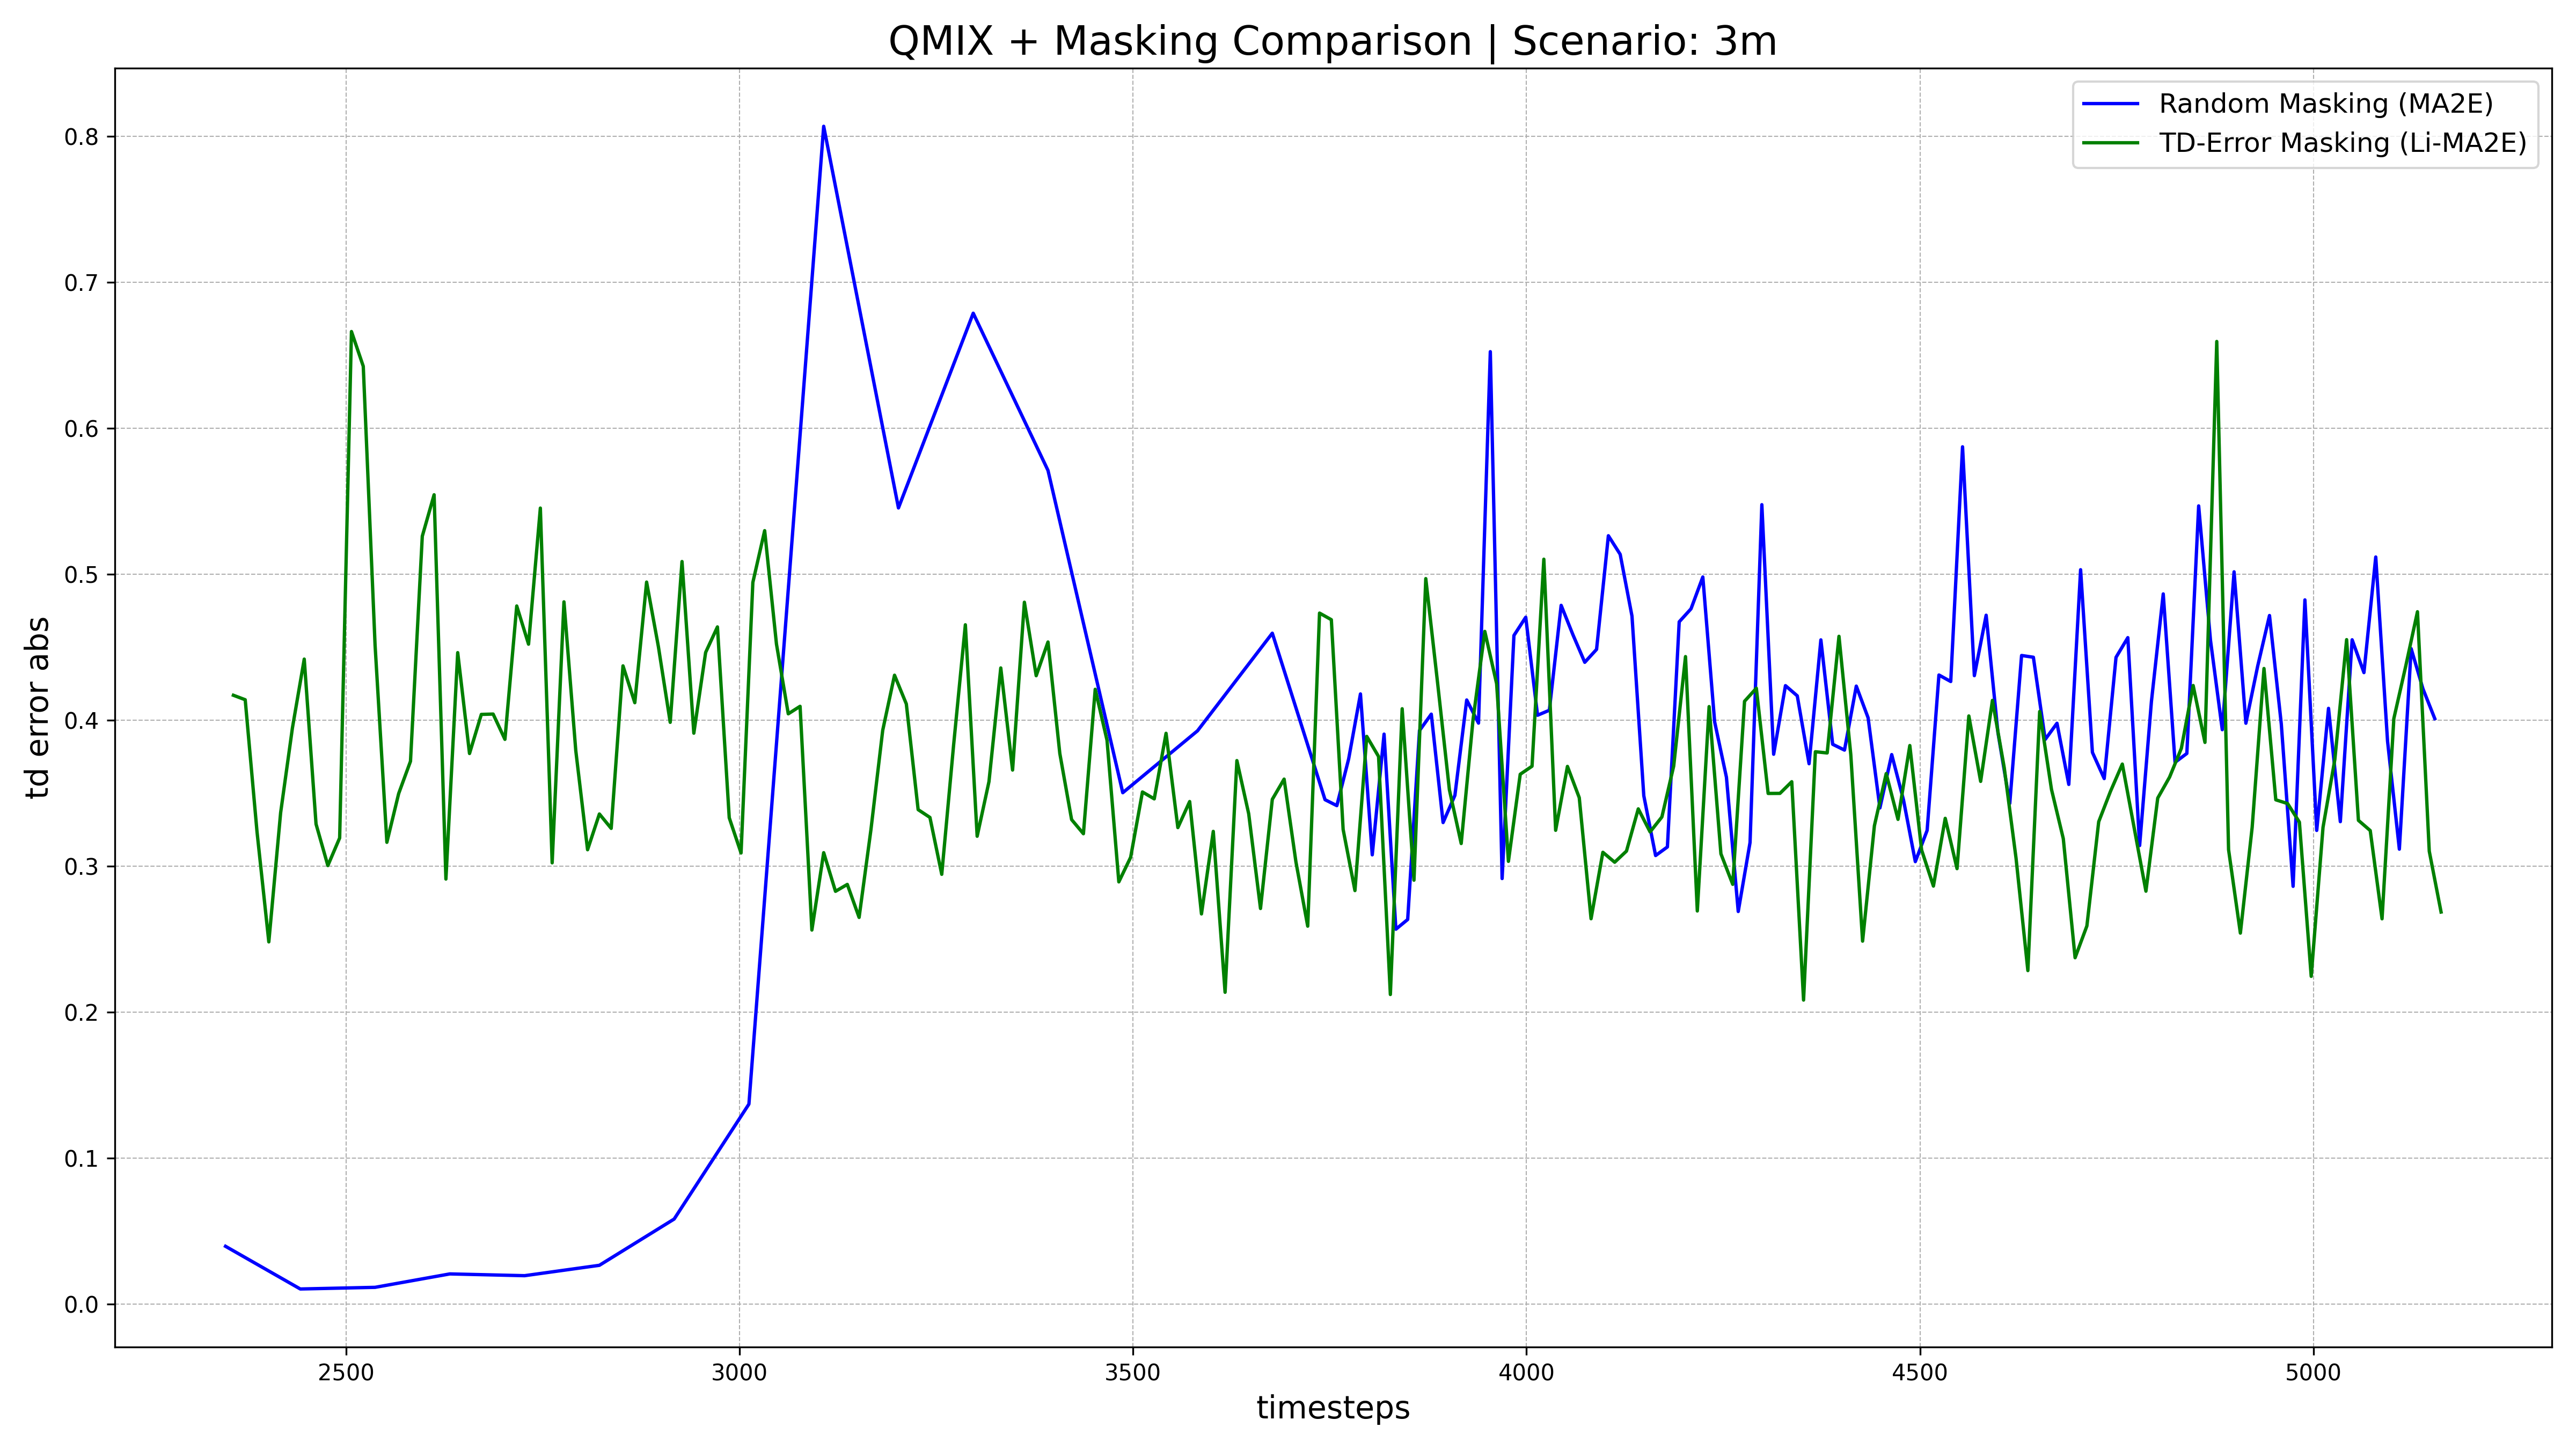
\includegraphics[width=0.8\textwidth]{images_pfe/results_td_error_abs/comparison_plot_3m.png}
%     \caption{Mean absolute TD-error on the \texttt{3m} scenario.}
%     \label{fig:3m_td_error}
% \end{figure}

% \paragraph{Analysis}
% In the \texttt{3m} scenario, the TD-error for the Random Masking baseline (blue line) starts low but spikes dramatically after 3000 timesteps, indicating a period of high instability as it learns. In contrast, our LI-MA2E method (green line) maintains a consistently lower and more stable TD-error throughout the same period. This suggests that our intelligent masking curriculum helps prevent these learning instabilities.

% %-------------------------------------------------
% \subsection{Scenario: \texttt{8m}}
% %-------------------------------------------------

% \begin{figure}[H]
%     \centering
%     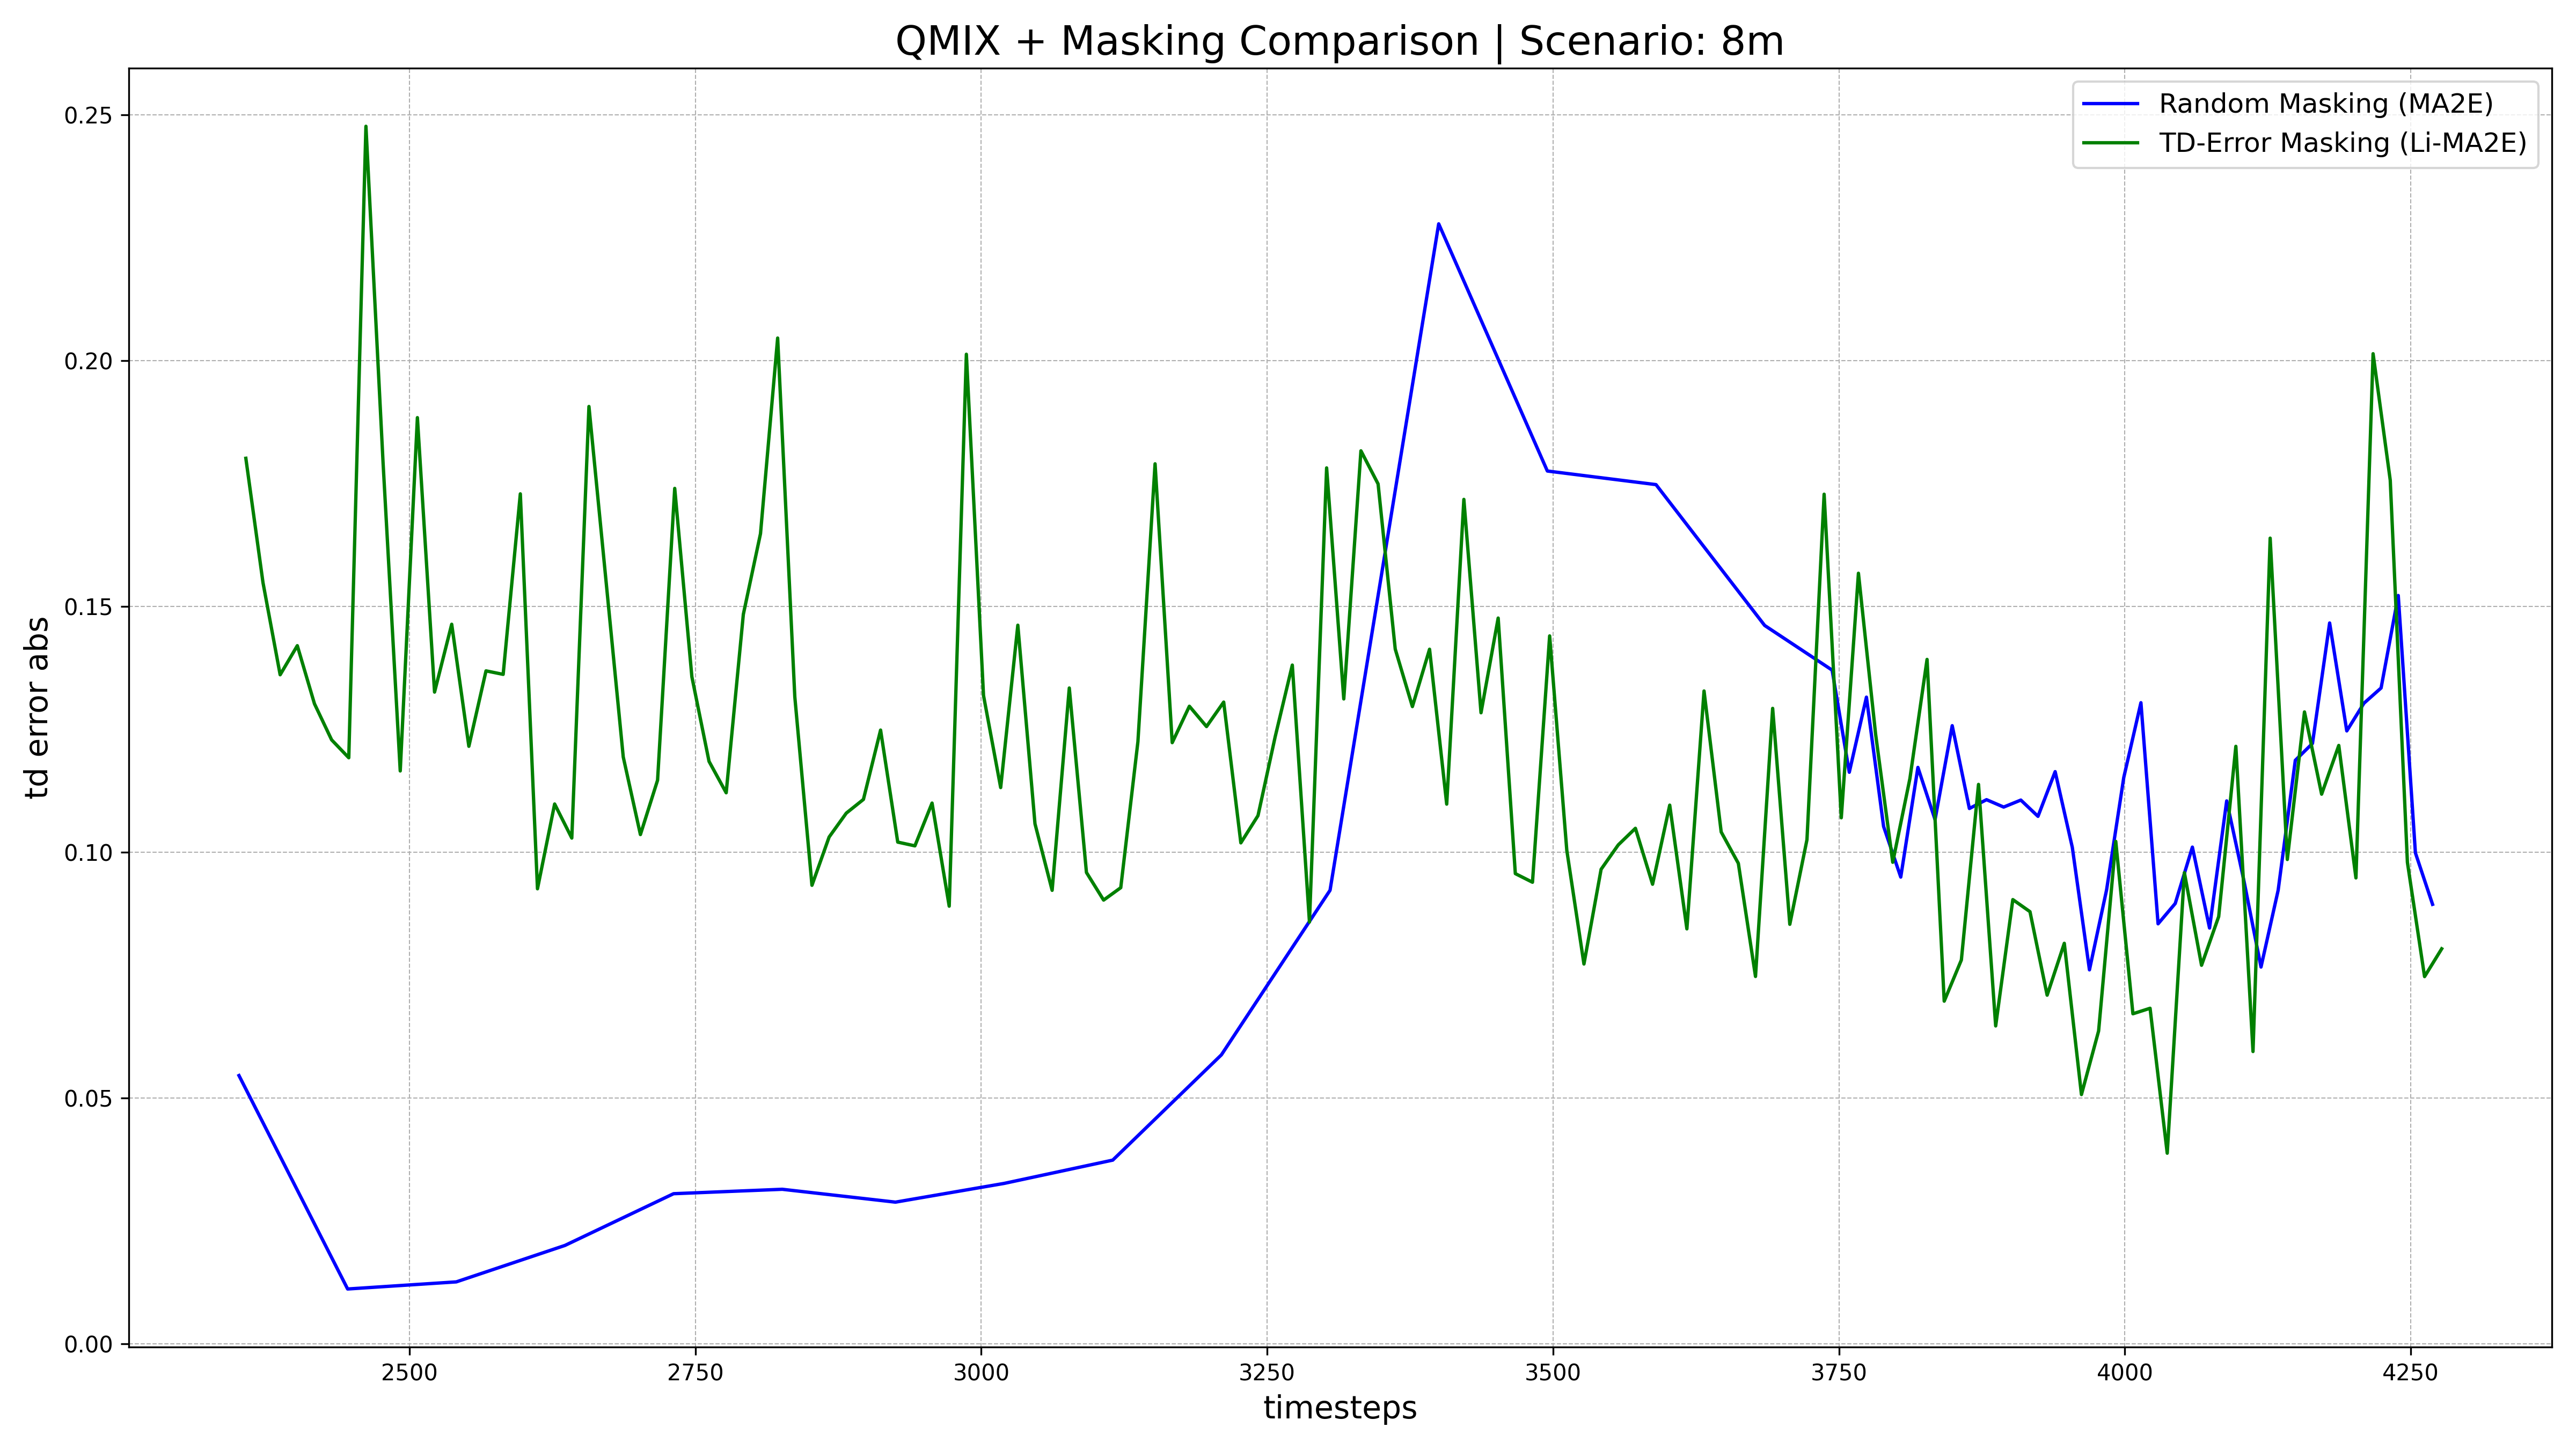
\includegraphics[width=0.8\textwidth]{images_pfe/results_td_error_abs/comparison_plot_8m.png}
%     \caption{Mean absolute TD-error on the \texttt{8m} scenario.}
%     \label{fig:8m_td_error}
% \end{figure}

% \paragraph{Analysis}
% The TD-error plot for the \texttt{8m} scenario shows a similar trend. The Random Masking baseline (blue line) exhibits a large spike in error around 3400 timesteps, signifying a significant learning challenge. Our LI-MA2E framework (green line), however, maintains a much more stable and consistently lower TD-error, effectively navigating the learning process without the same degree of instability.

% %-------------------------------------------------
% \subsection{Scenario: \texttt{3s\_vs\_3z}}
% %-------------------------------------------------

% \begin{figure}[H]
%     \centering
%     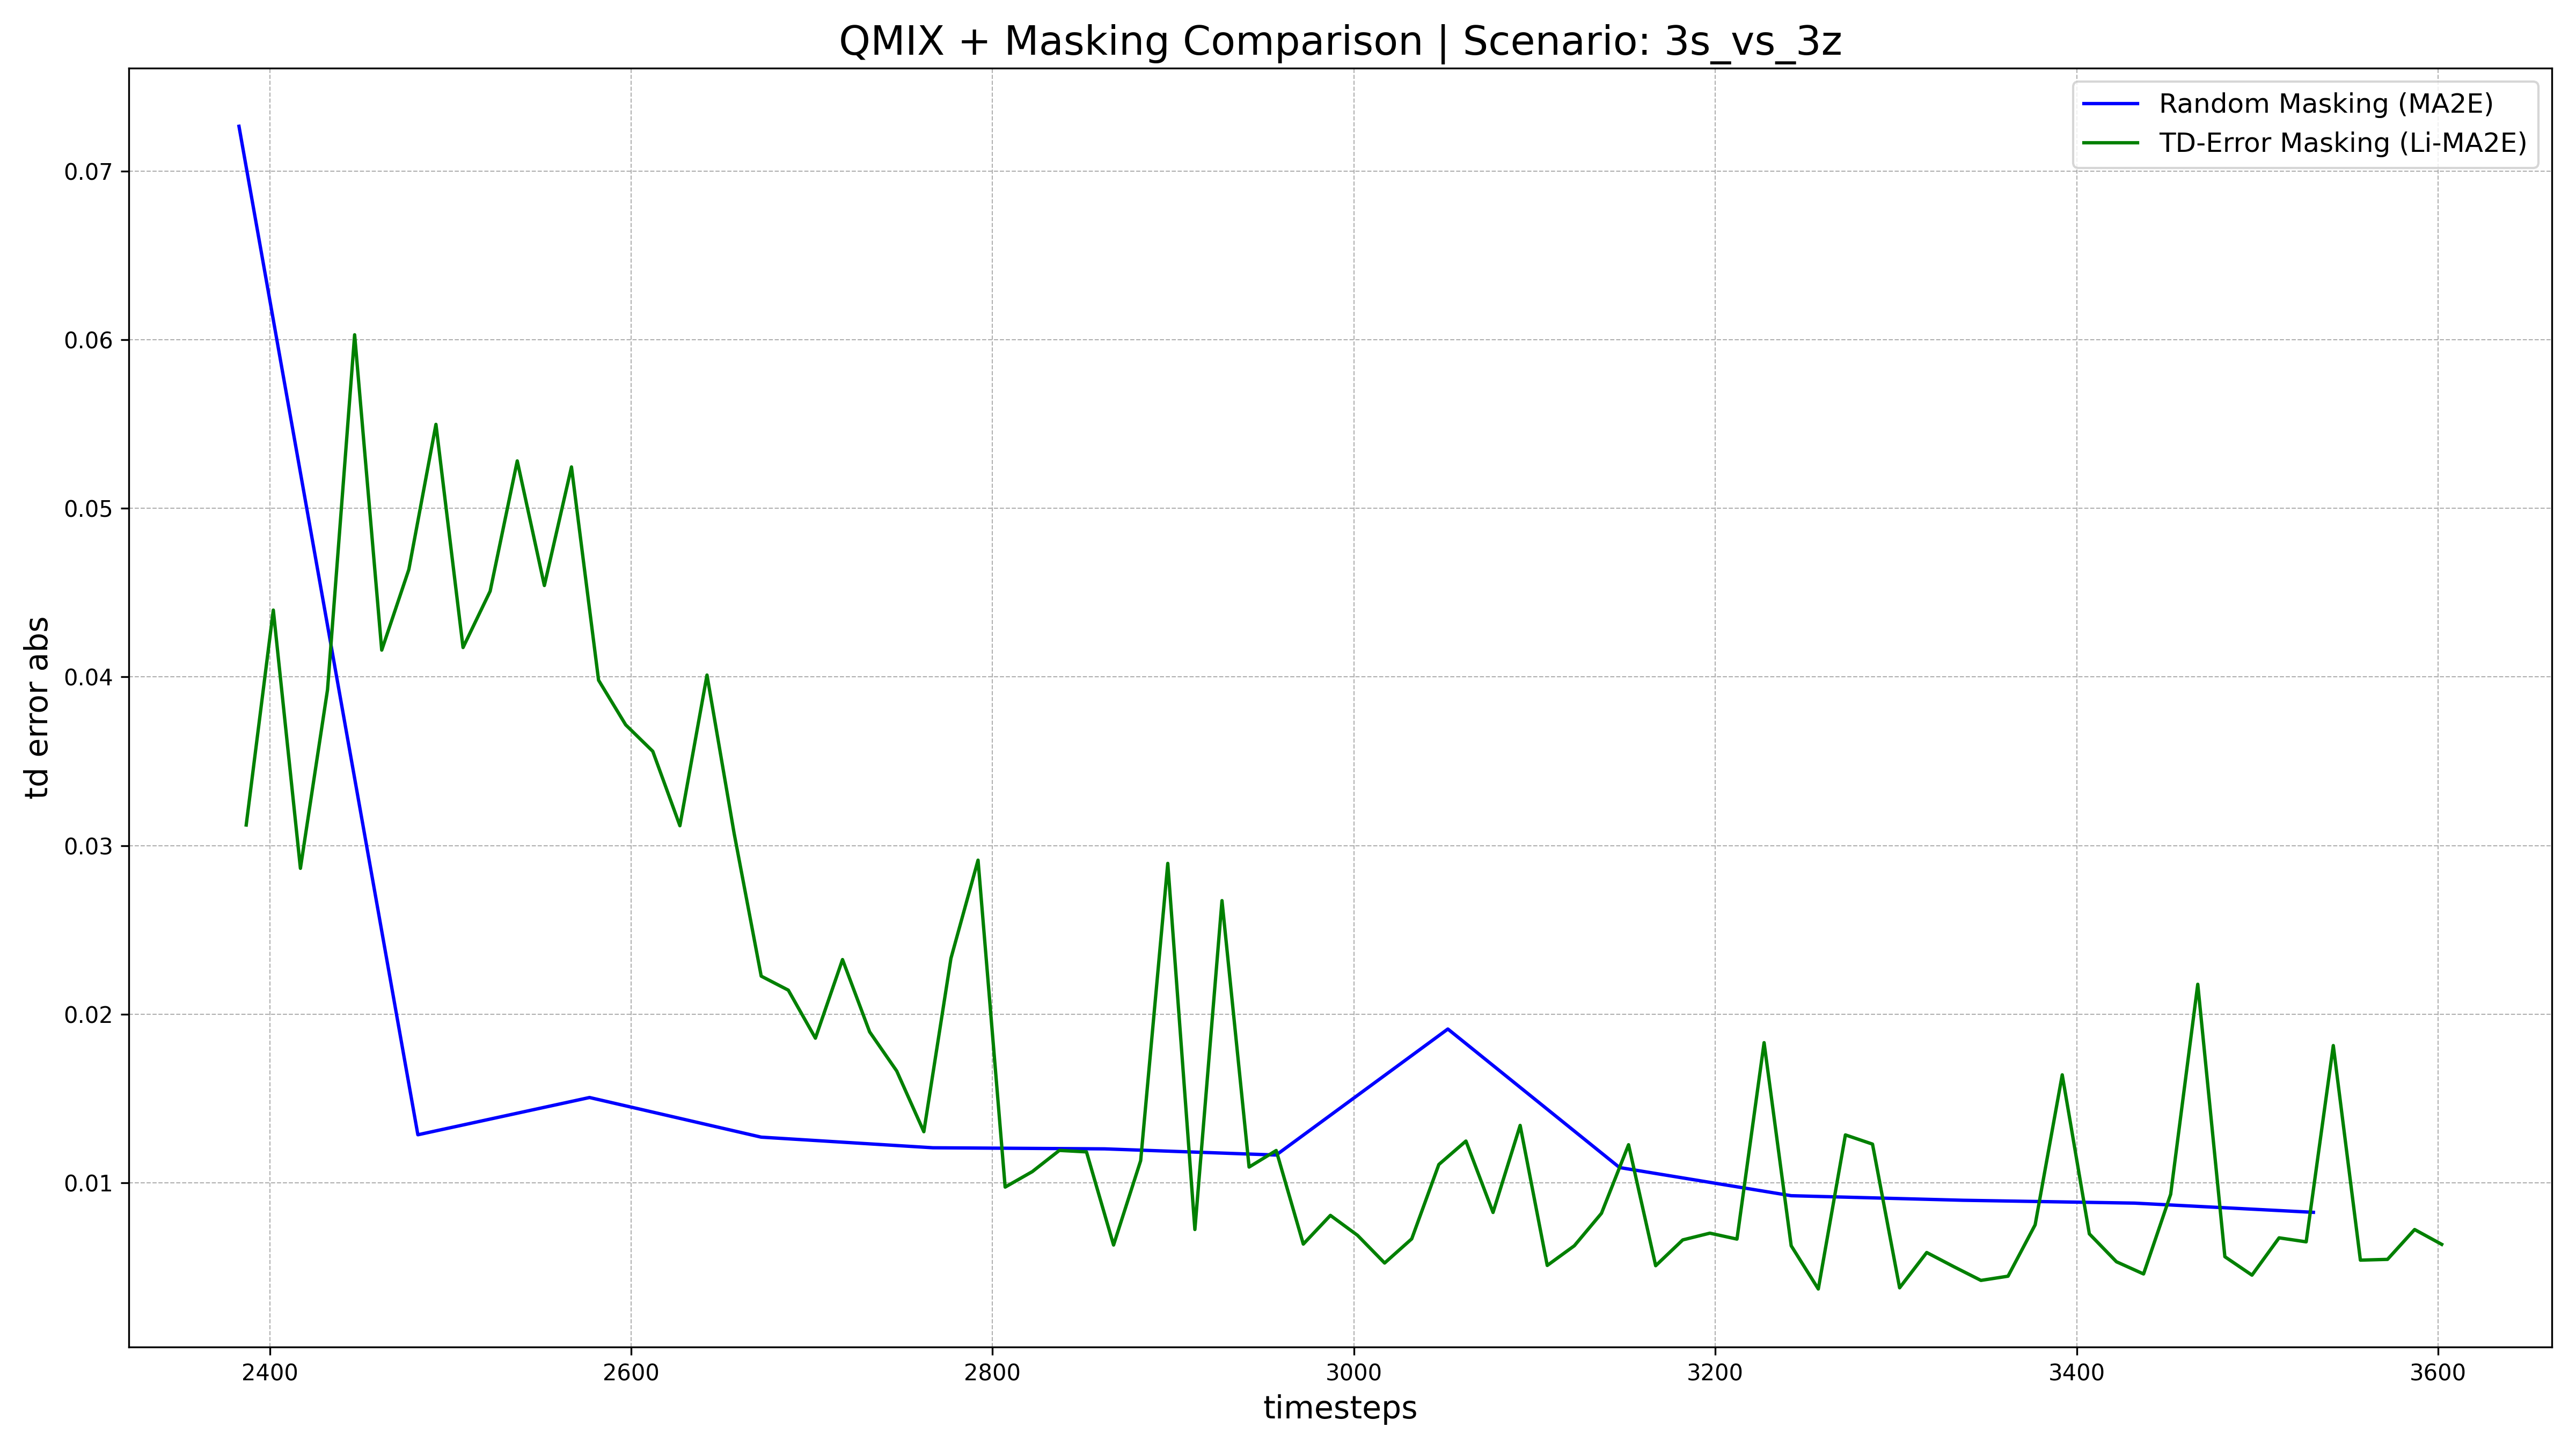
\includegraphics[width=0.8\textwidth]{images_pfe/results_td_error_abs/comparison_plot_3s_vs_3z.png}
%     \caption{Mean absolute TD-error on the  \texttt{3s\_vs\_3z} scenario.}
%     \label{fig:3s_vs_3z_td_error}
% \end{figure}

% \paragraph{Analysis}
% In the  \texttt{3s\_vs\_3z} scenario, the initial TD-error for the baseline (blue line) is very high before it sharply drops and stabilizes at a low value. Our LI-MA2E method (green line) shows a more controlled descent, and while it exhibits more variance, it consistently pushes the error to a lower floor than the baseline after 3000 timesteps. This demonstrates a more effective error reduction in the long run.

% %-------------------------------------------------
% \subsection{Scenario: \texttt{3s\_vs\_4z}}
% %-------------------------------------------------

% \begin{figure}[H]
%     \centering
%     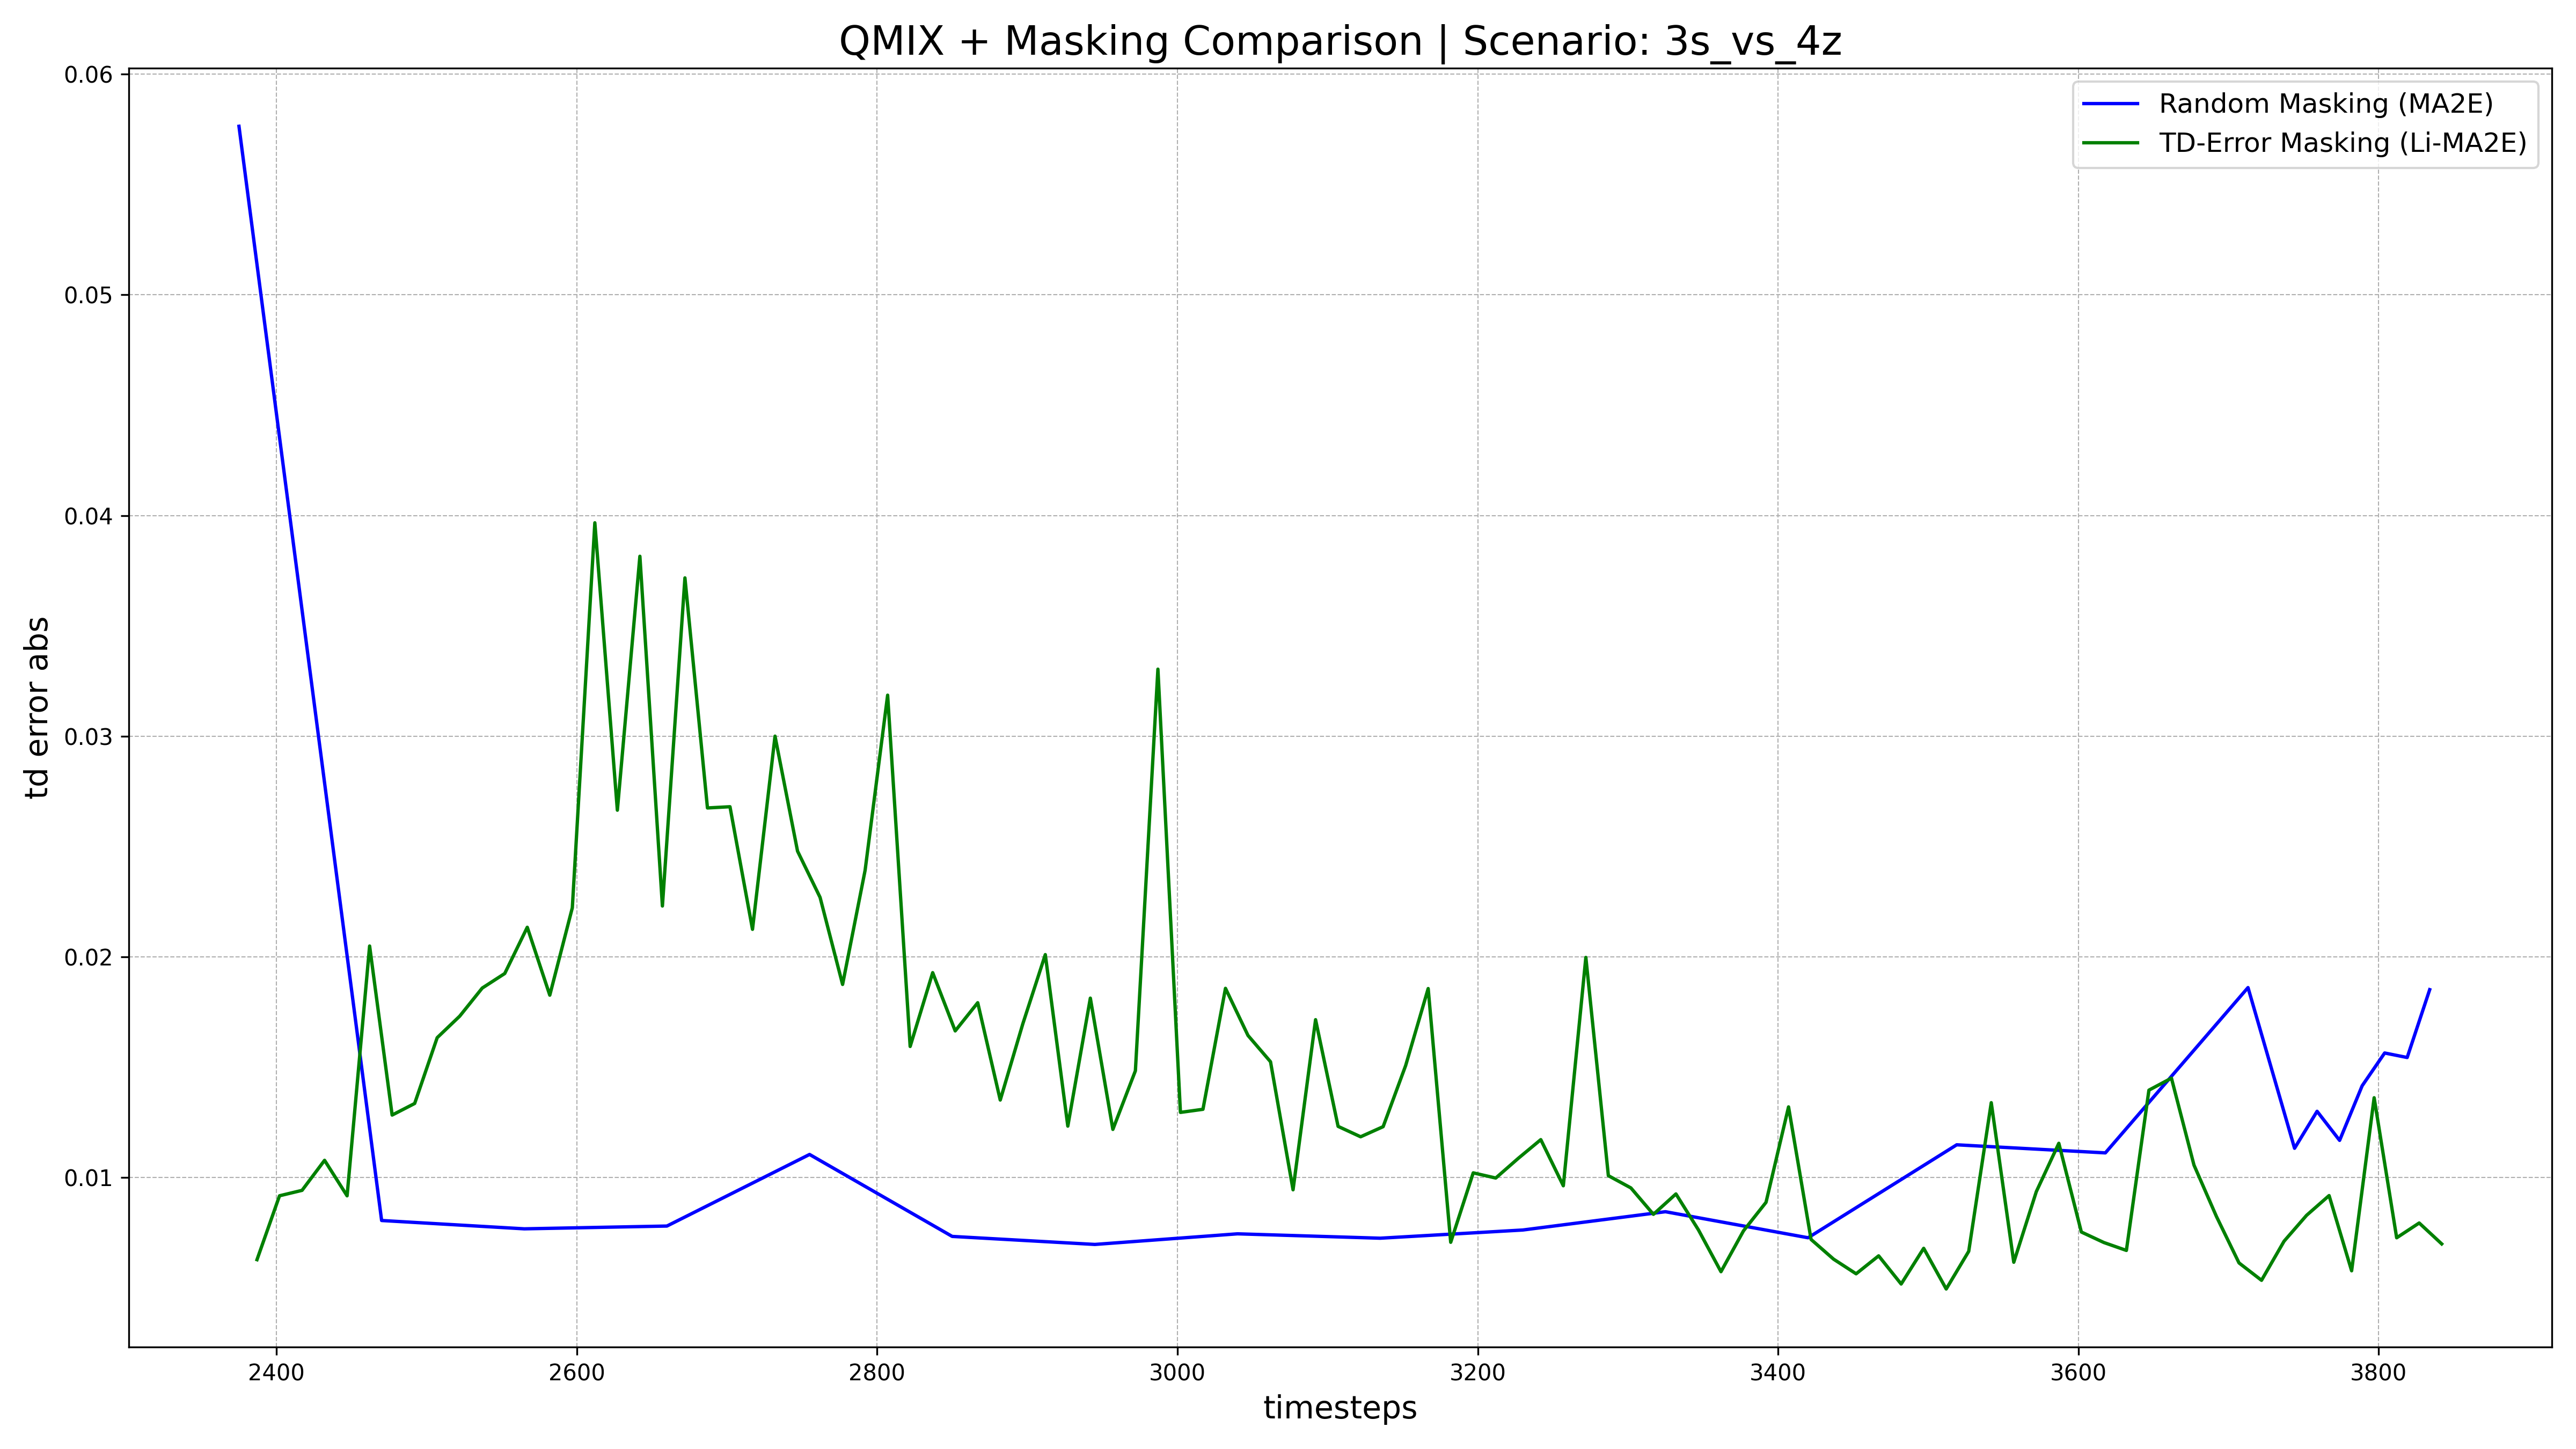
\includegraphics[width=0.8\textwidth]{images_pfe/results_td_error_abs/comparison_plot_3s_vs_4z.png}
%     \caption{Mean absolute TD-error on the `3s\_vs\_4z` scenario.}
%     \label{fig:3s_vs_4z_td_error}
% \end{figure}

% \paragraph{Analysis}
% The results on  \texttt{3s\_vs\_4z} are particularly telling. The baseline's TD-error (blue line) remains stubbornly high for a long period before slowly decreasing. In contrast, the LI-MA2E's TD-error (green line), while initially volatile, is driven down much more effectively and consistently remains at a lower level than the baseline. This directly supports the finding that LI-MA2E learns a higher-quality policy, as it is more successful at minimizing the underlying prediction error.

% %-------------------------------------------------
% \subsection{Scenario: \texttt{3s\_vs\_5z}}
% %-------------------------------------------------

% \begin{figure}[H]
%     \centering
%     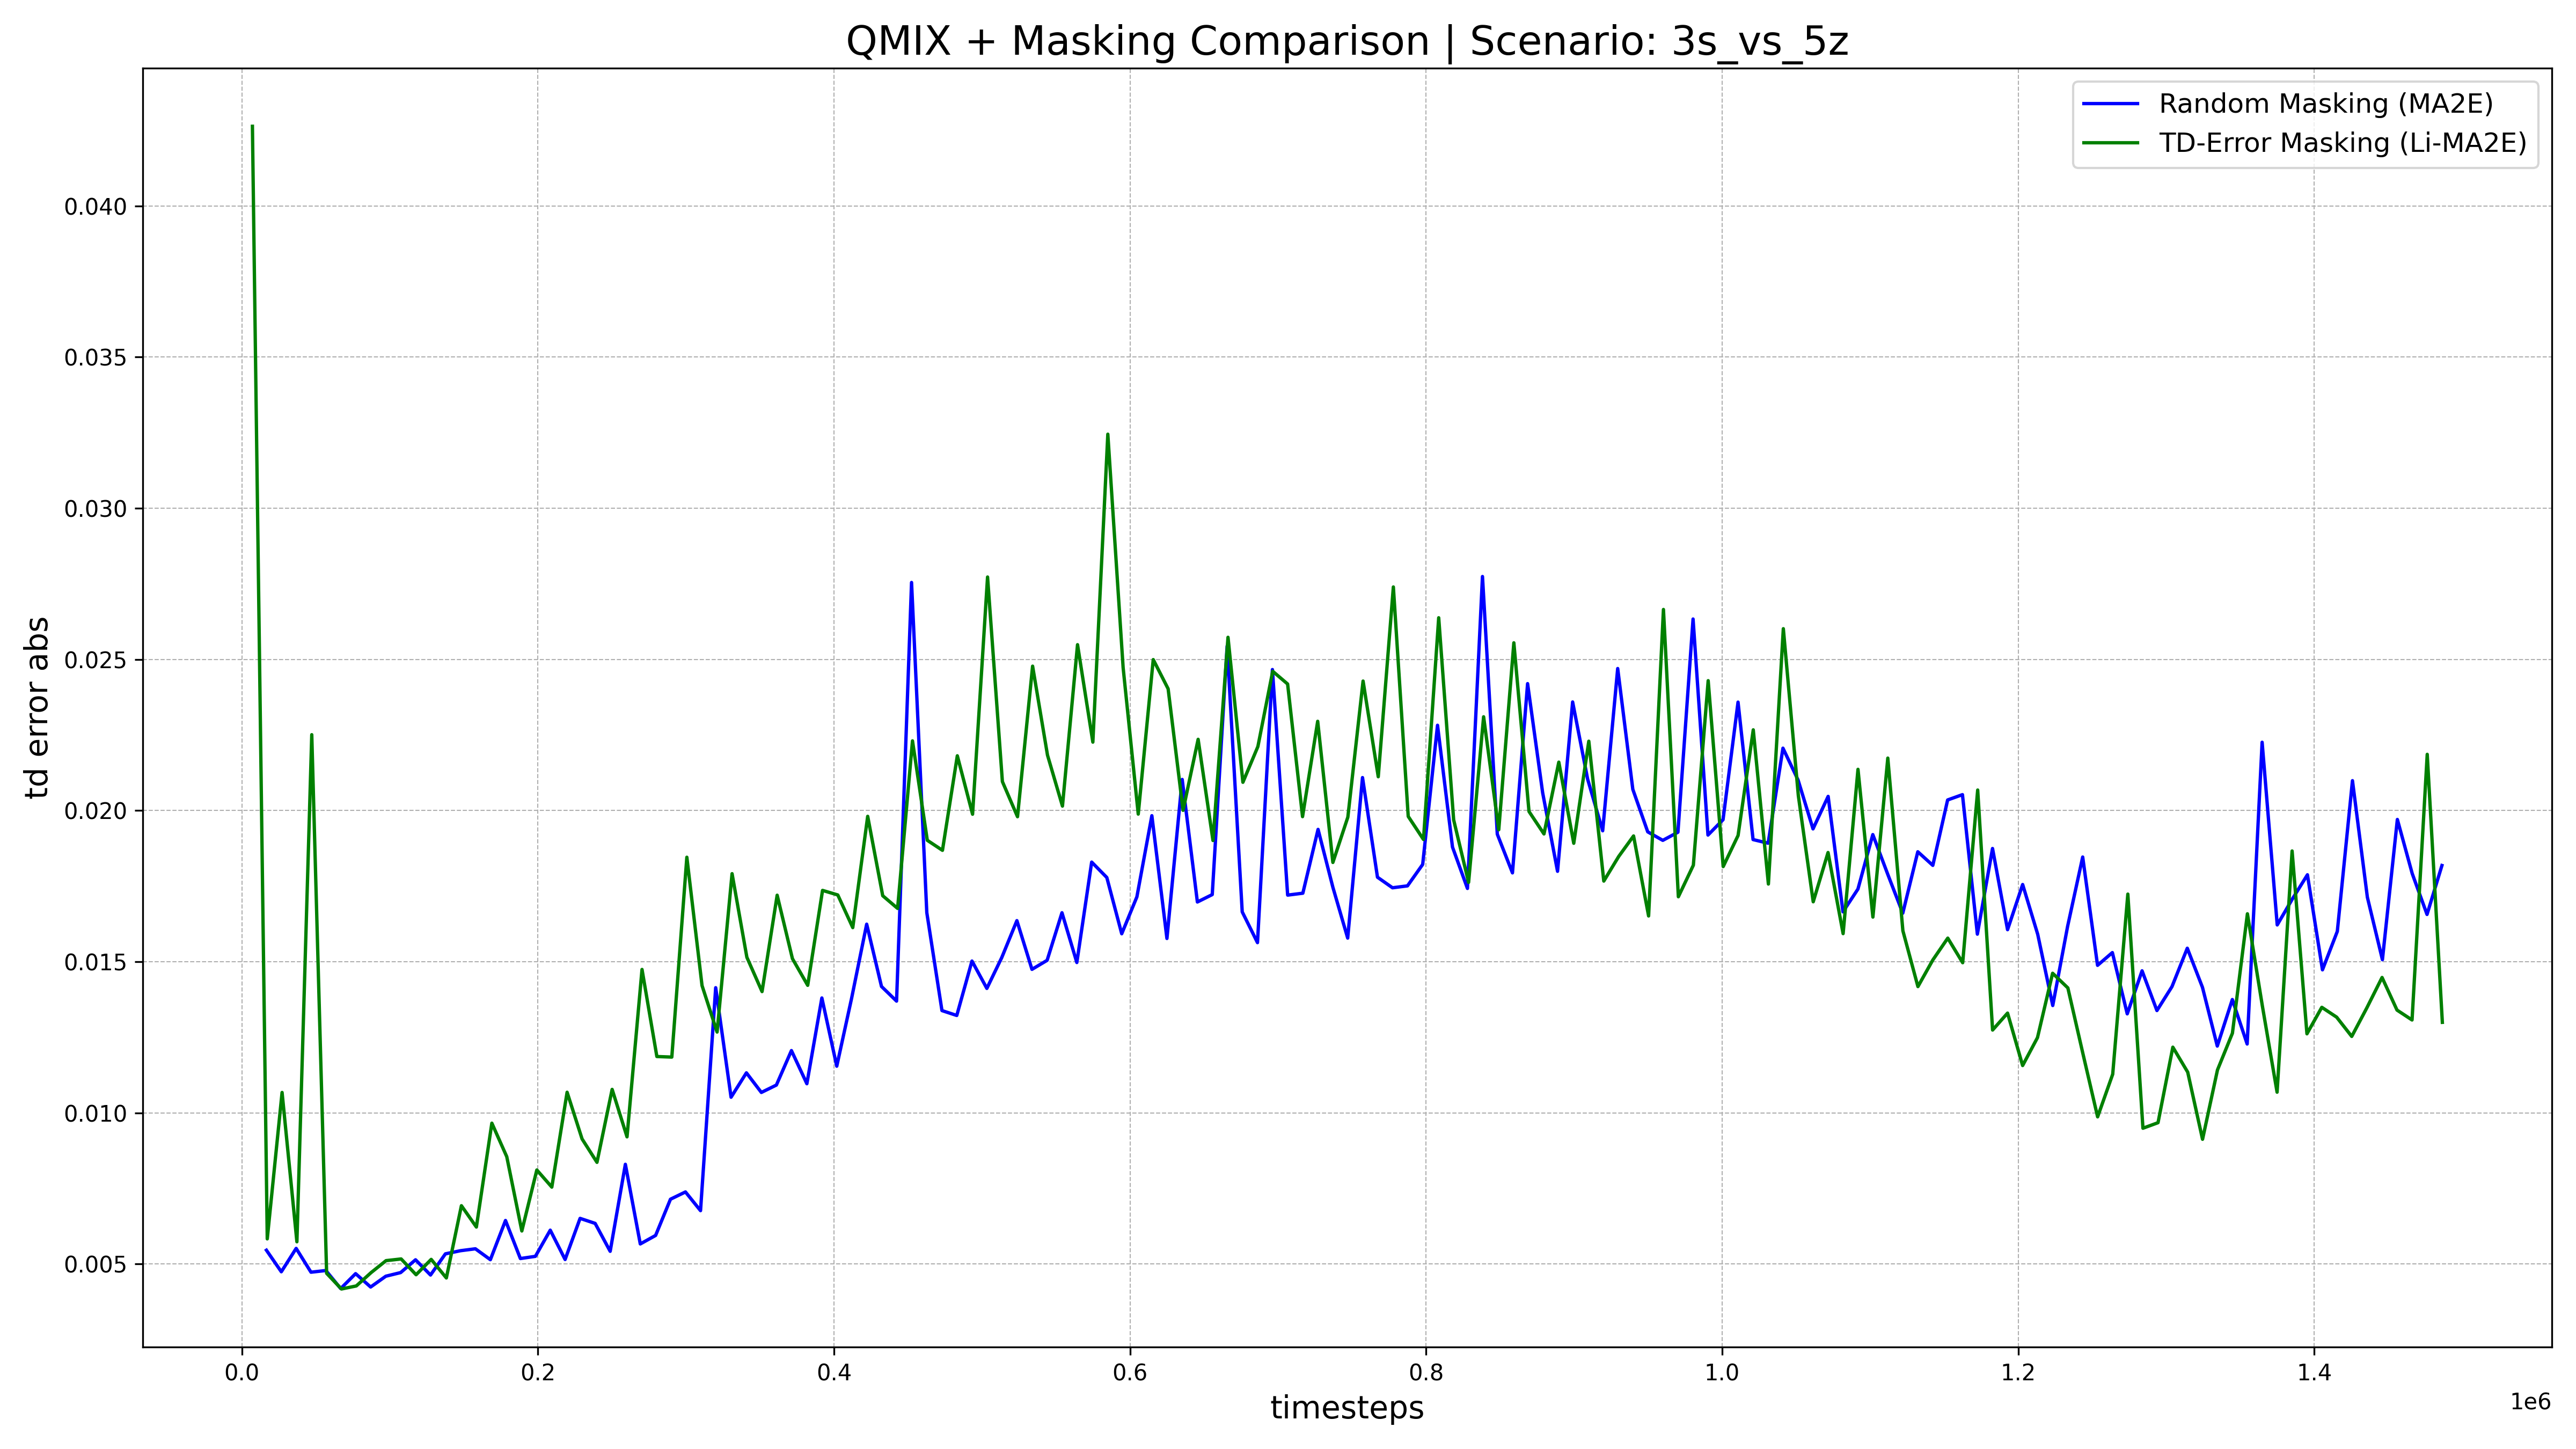
\includegraphics[width=0.8\textwidth]{images_pfe/results_td_error_abs/comparison_plot_3s_vs_5z.png}
%     \caption{Mean absolute TD-error on the \texttt{3s\_vs\_5z} scenario.}
%     \label{fig:3s_vs_5z_td_error}
% \end{figure}

% \paragraph{Analysis}
% On the difficult \texttt{3s\_vs\_5z} map, our LI-MA2E method (green line) again demonstrates its ability to control and reduce error more effectively than the baseline (blue line). After an initial spike, the green line is consistently suppressed, while the blue line remains higher for longer. This shows that by focusing on the agents with high error, our method creates a curriculum that actively minimizes that error across the team, leading to a more stable and efficient learning process. This stability is the reason LI-MA2E achieves higher returns and avoids the policy degradation seen in the baseline.
\chapter{Analysis of Learning Stability}
\section{Analysis of Mean Absolute TD-error}
\label{app:td_error_abs_analysis}

This appendix provides a direct analysis of the learning process by visualizing the mean absolute TD-error. This metric offers insight into the stability and convergence of the agents' underlying value functions. A lower, more stable TD-error indicates that the agents are making more accurate predictions and have learned a more reliable policy. Figure~\ref{fig:all_td_errors} compares our LI-MA2E framework against the baseline Random Masking across the tested SMAC scenarios.

\begin{figure}[H]
    \centering
    % Row 1 of plots
    \subfloat[Scenario: \texttt{3m}]{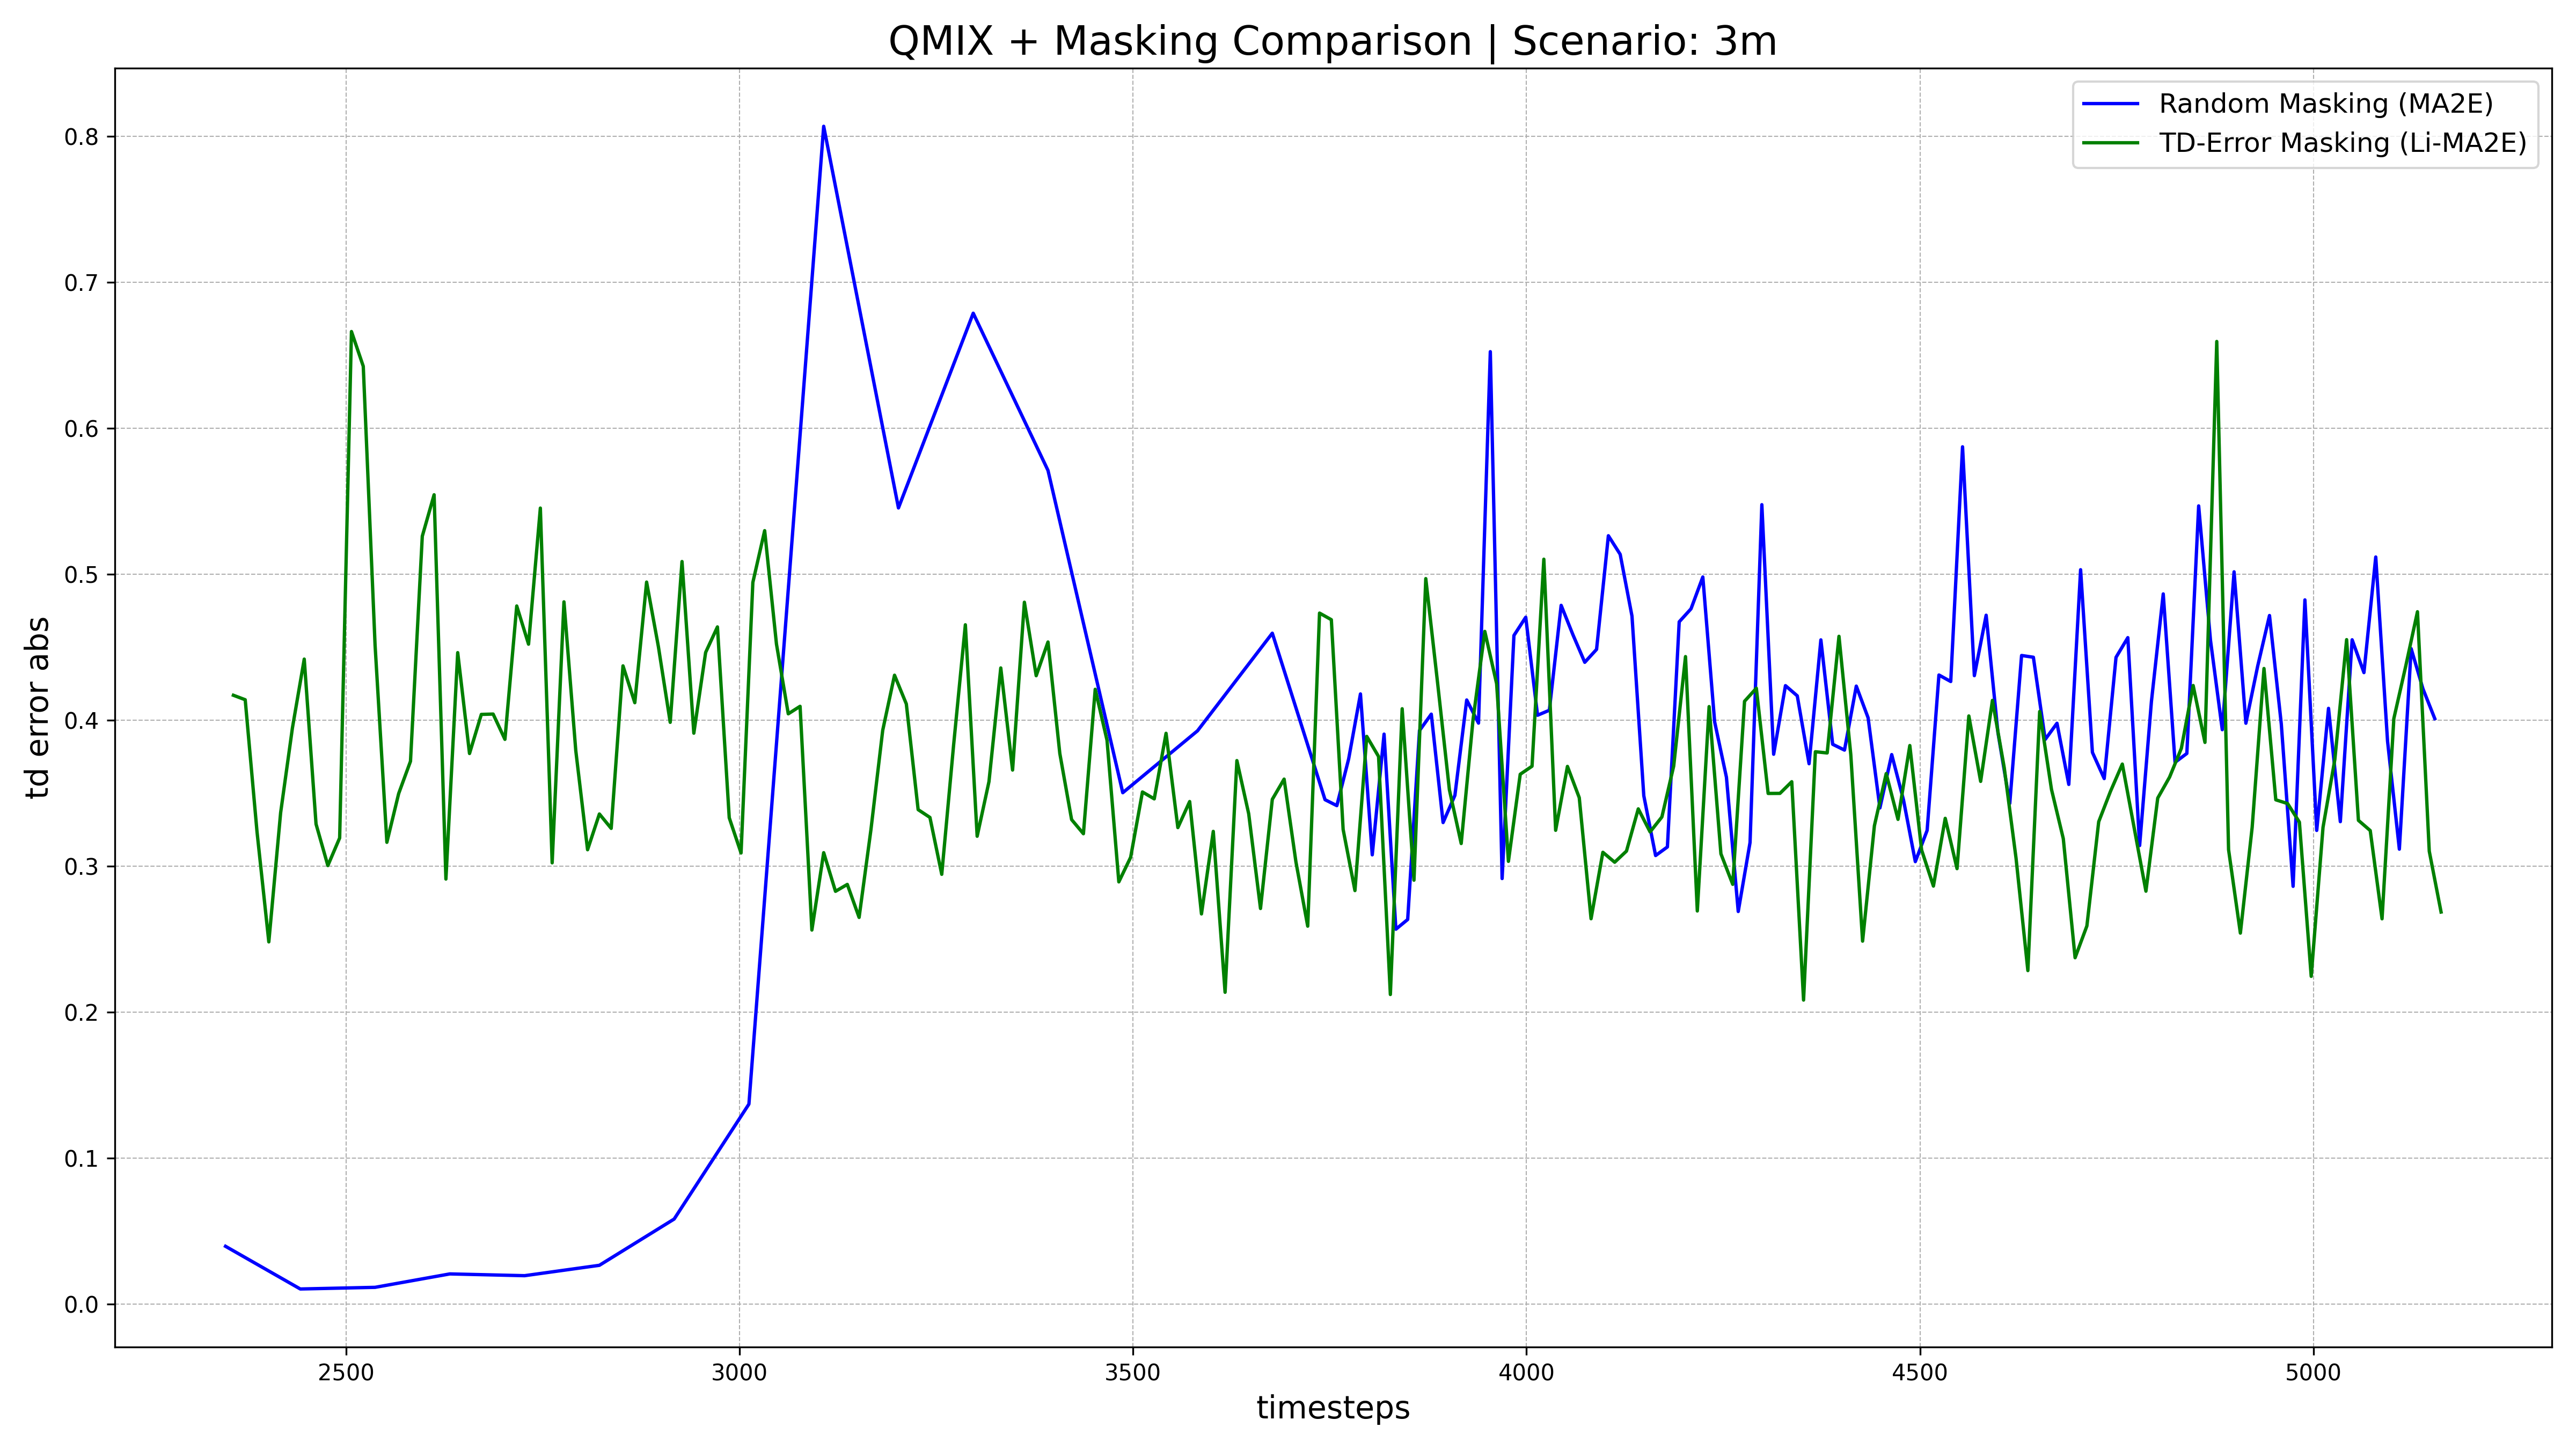
\includegraphics[width=0.32\textwidth]{images_pfe/results_td_error_abs/comparison_plot_3m.png}\label{fig:3m_td_error}}
    \hfill
    \subfloat[Scenario: \texttt{8m}]{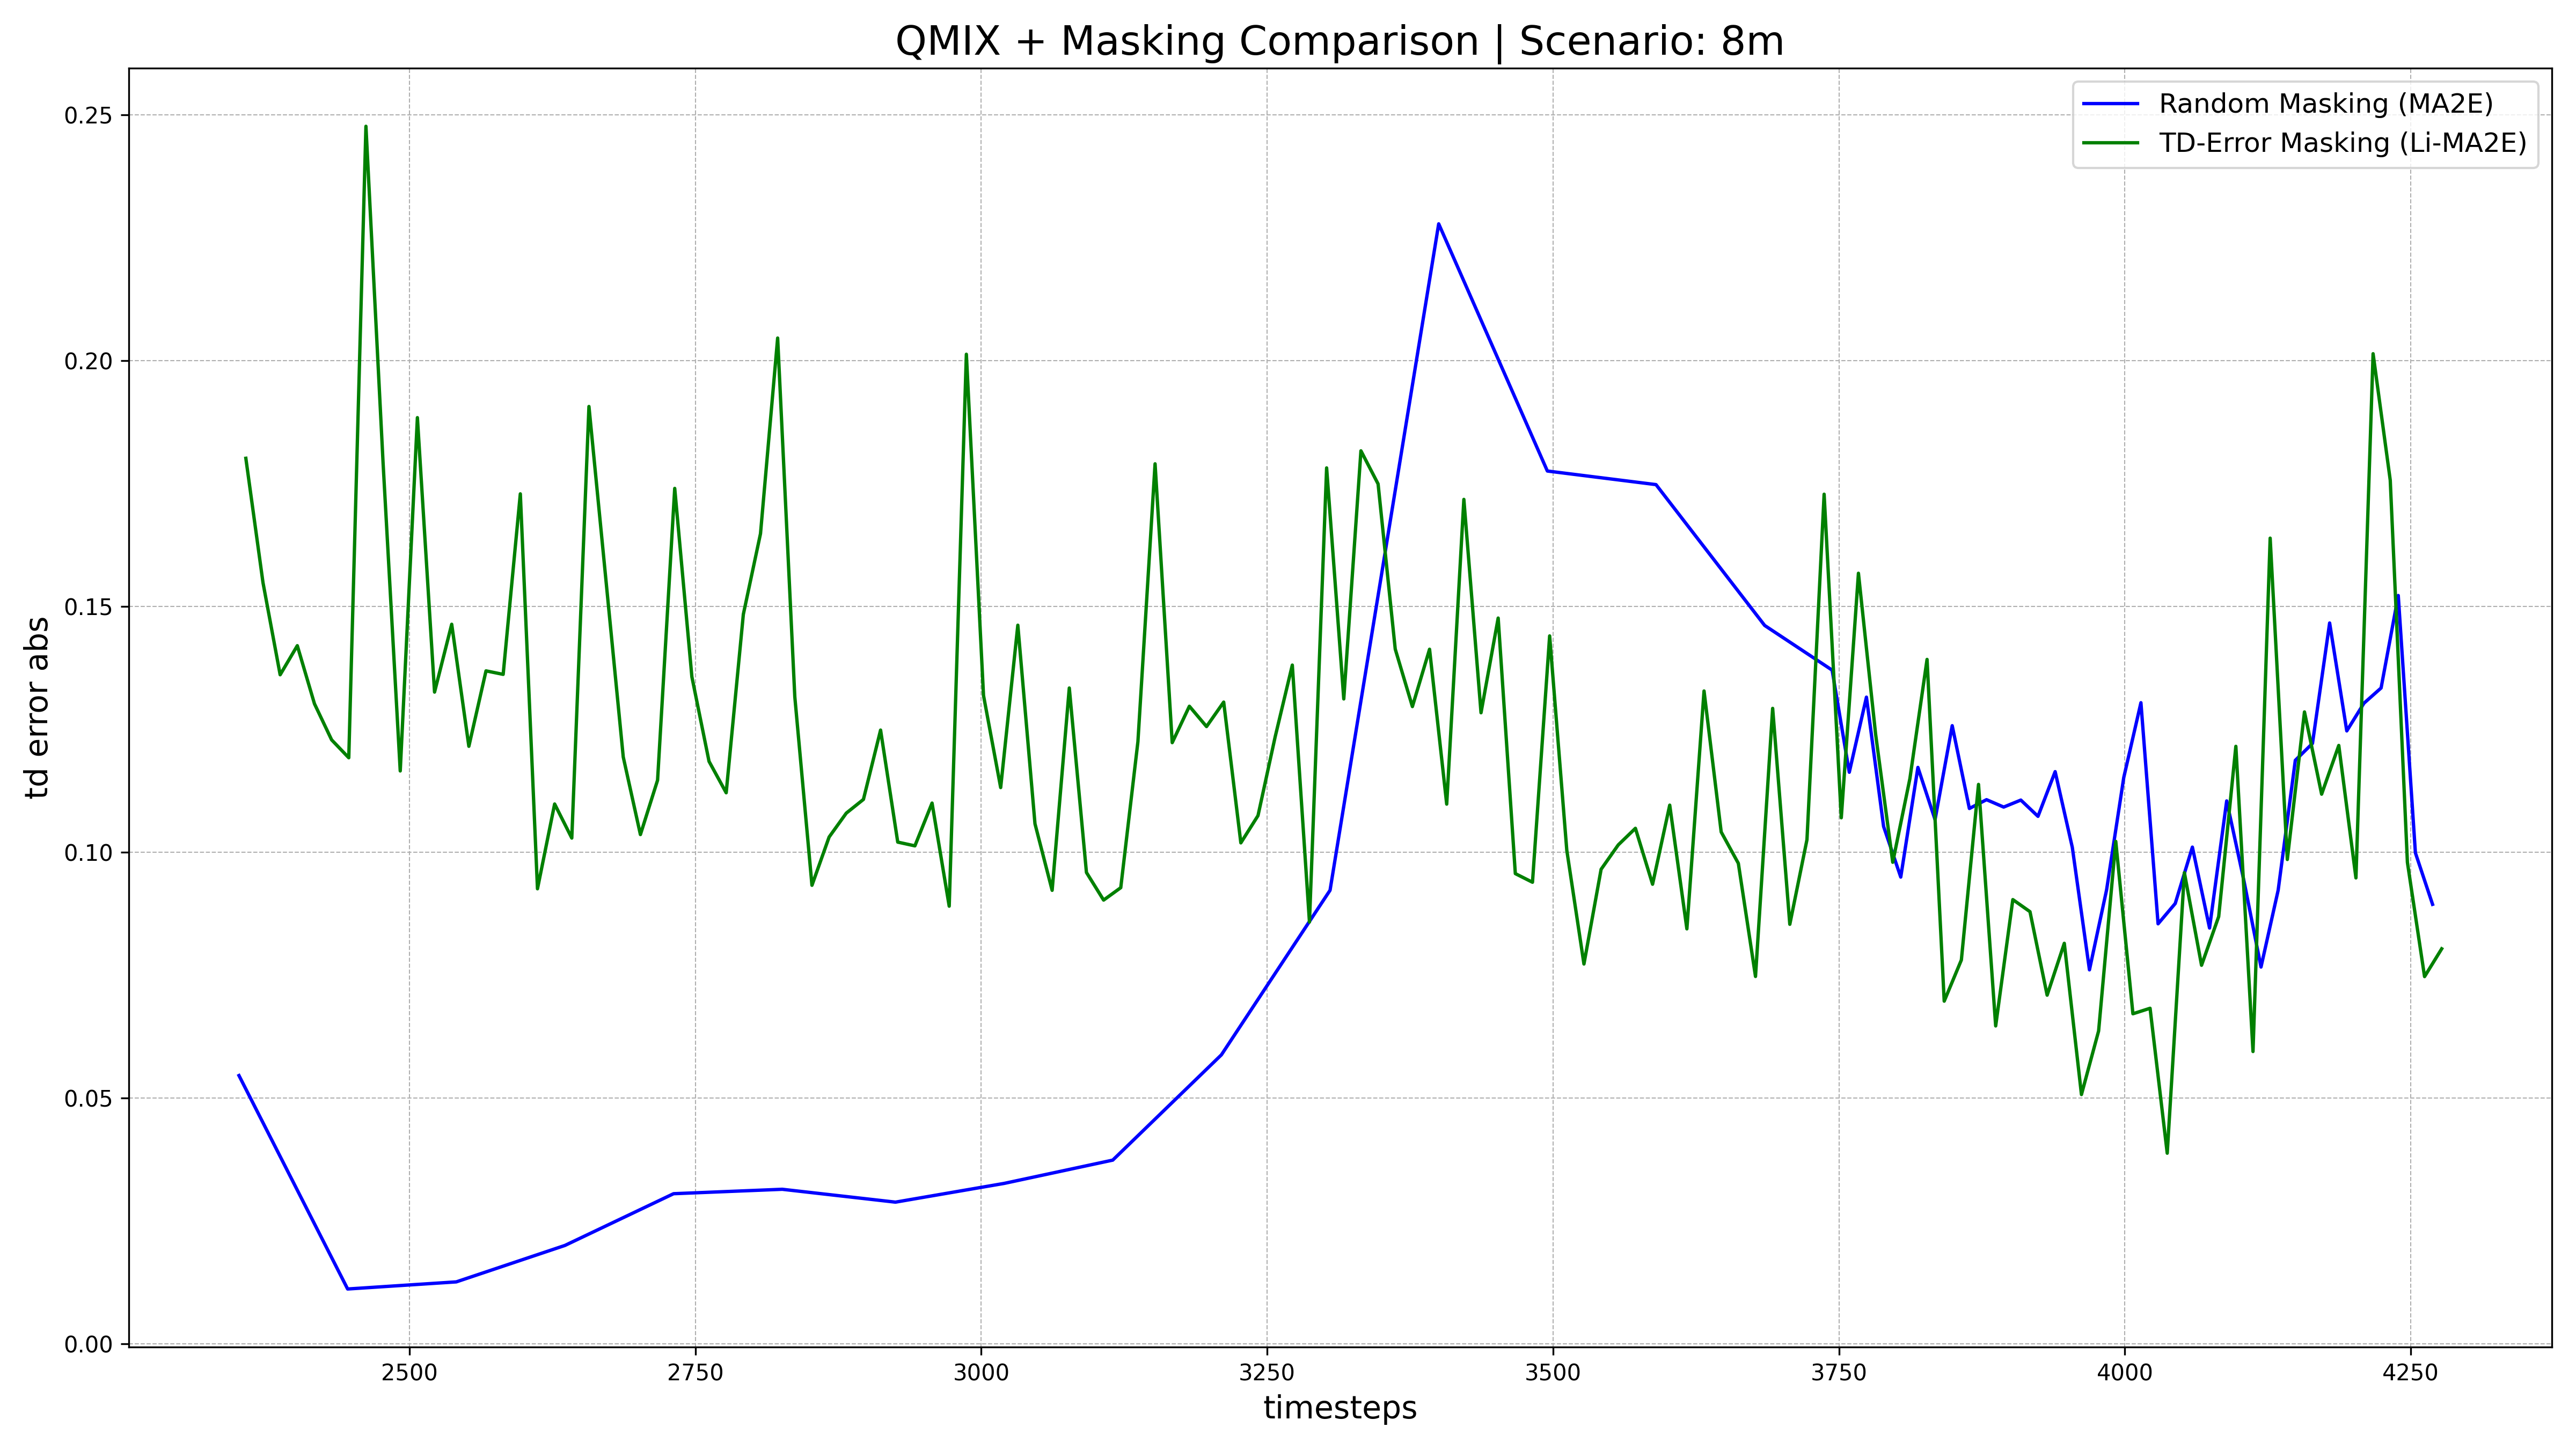
\includegraphics[width=0.32\textwidth]{images_pfe/results_td_error_abs/comparison_plot_8m.png}\label{fig:8m_td_error}}
    \hfill
    \subfloat[Scenario: \texttt{3s\_vs\_3z}]{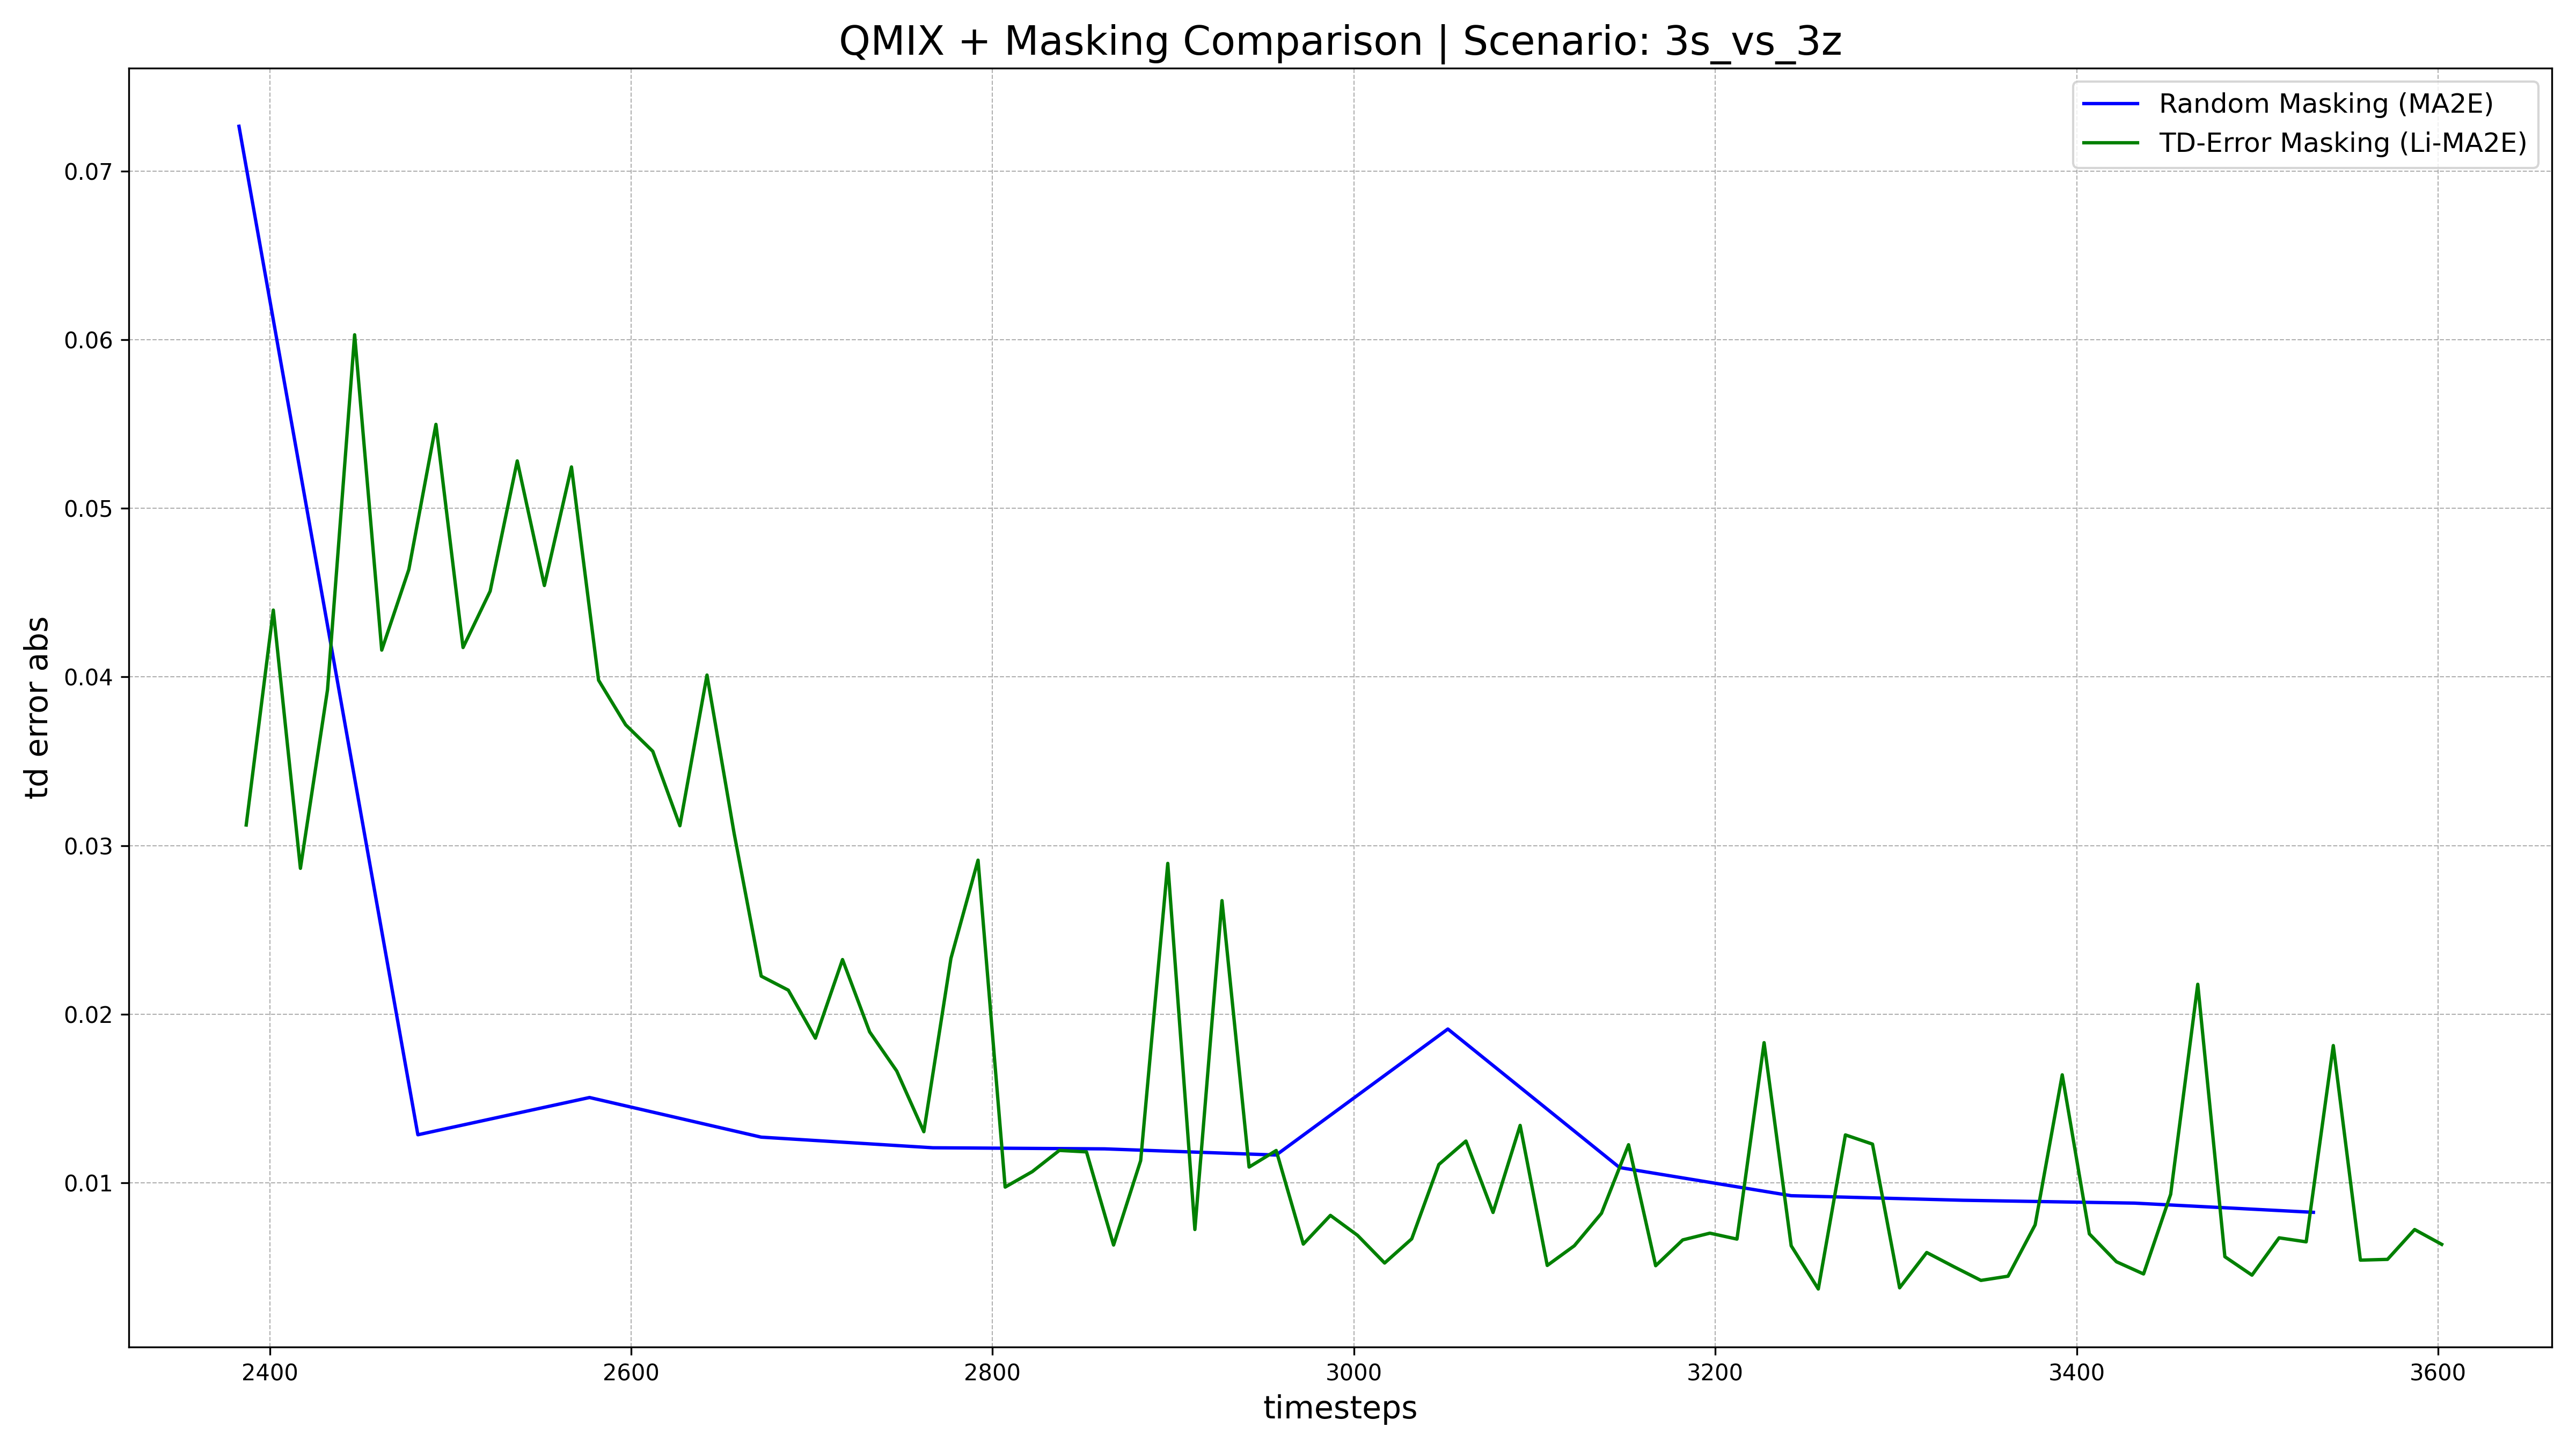
\includegraphics[width=0.32\textwidth]{images_pfe/results_td_error_abs/comparison_plot_3s_vs_3z.png}\label{fig:3s_vs_3z_td_error}}
    
    \vspace{1em} % Adds a little vertical space between rows
    
    % Row 2 of plots
    \subfloat[Scenario: \texttt{3s\_vs\_4z}]{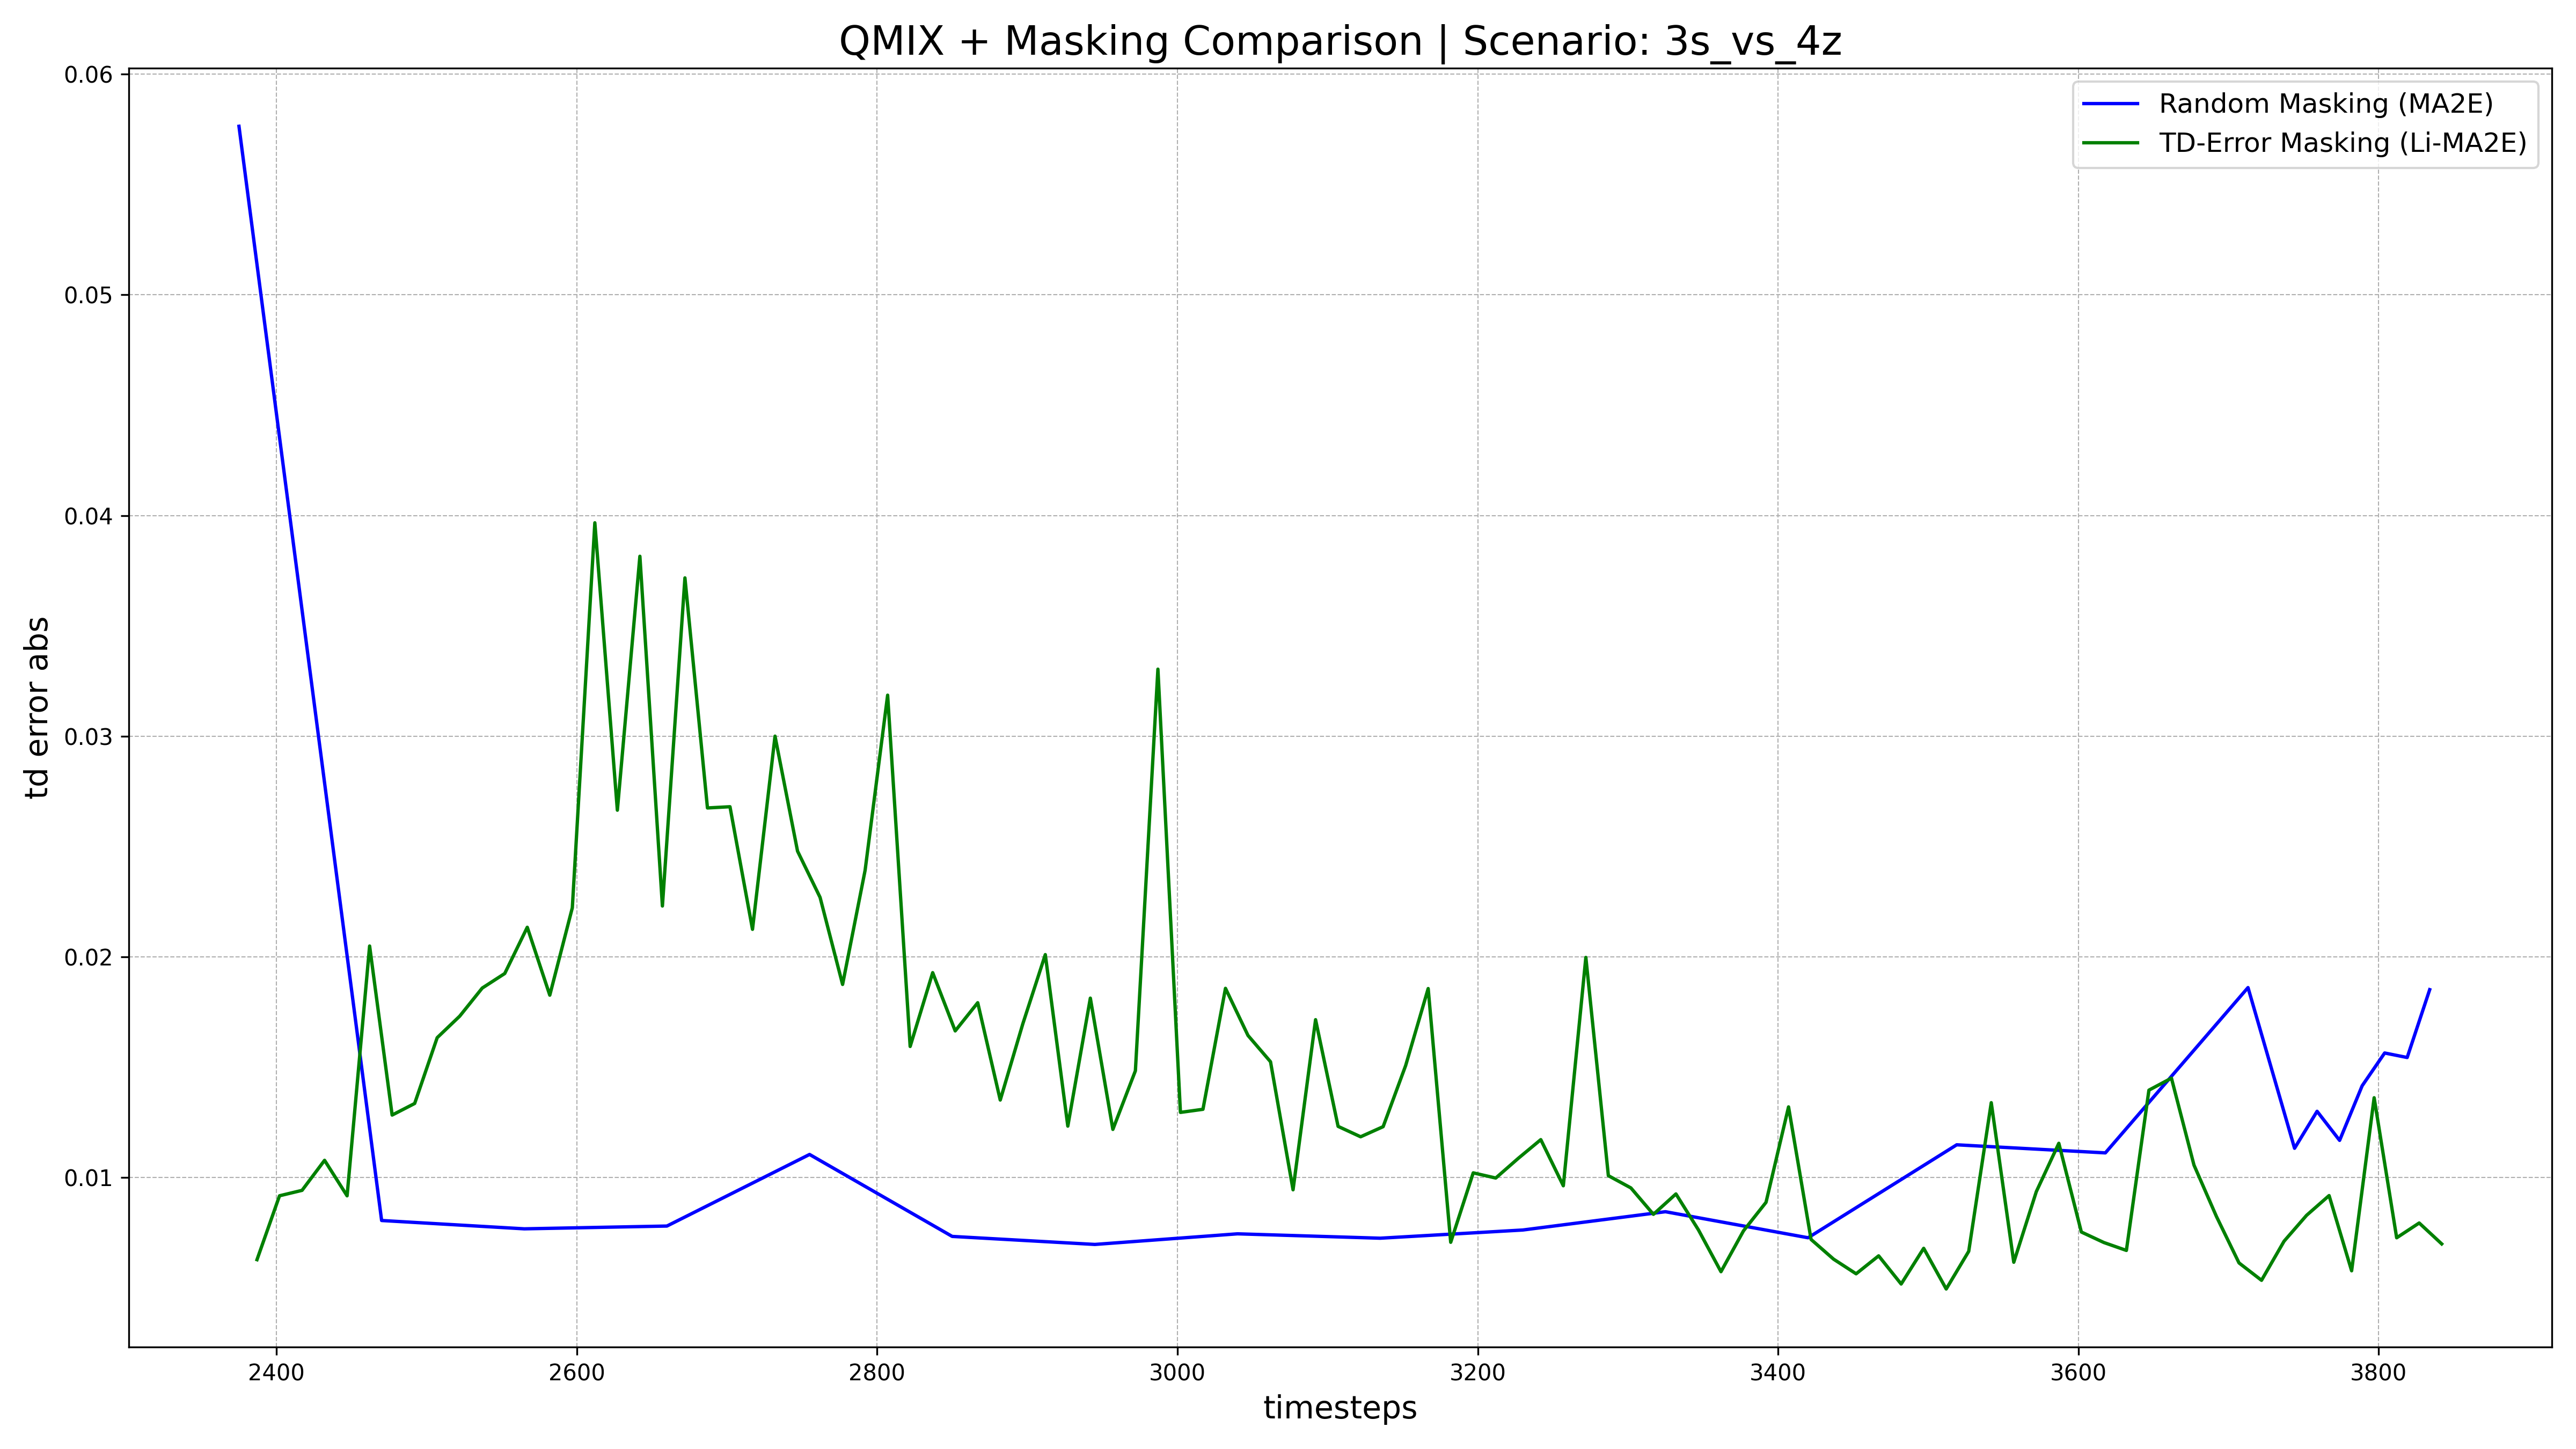
\includegraphics[width=0.32\textwidth]{images_pfe/results_td_error_abs/comparison_plot_3s_vs_4z.png}\label{fig:3s_vs_4z_td_error}}
    \hfill
    \subfloat[Scenario: \texttt{3s\_vs\_5z}]{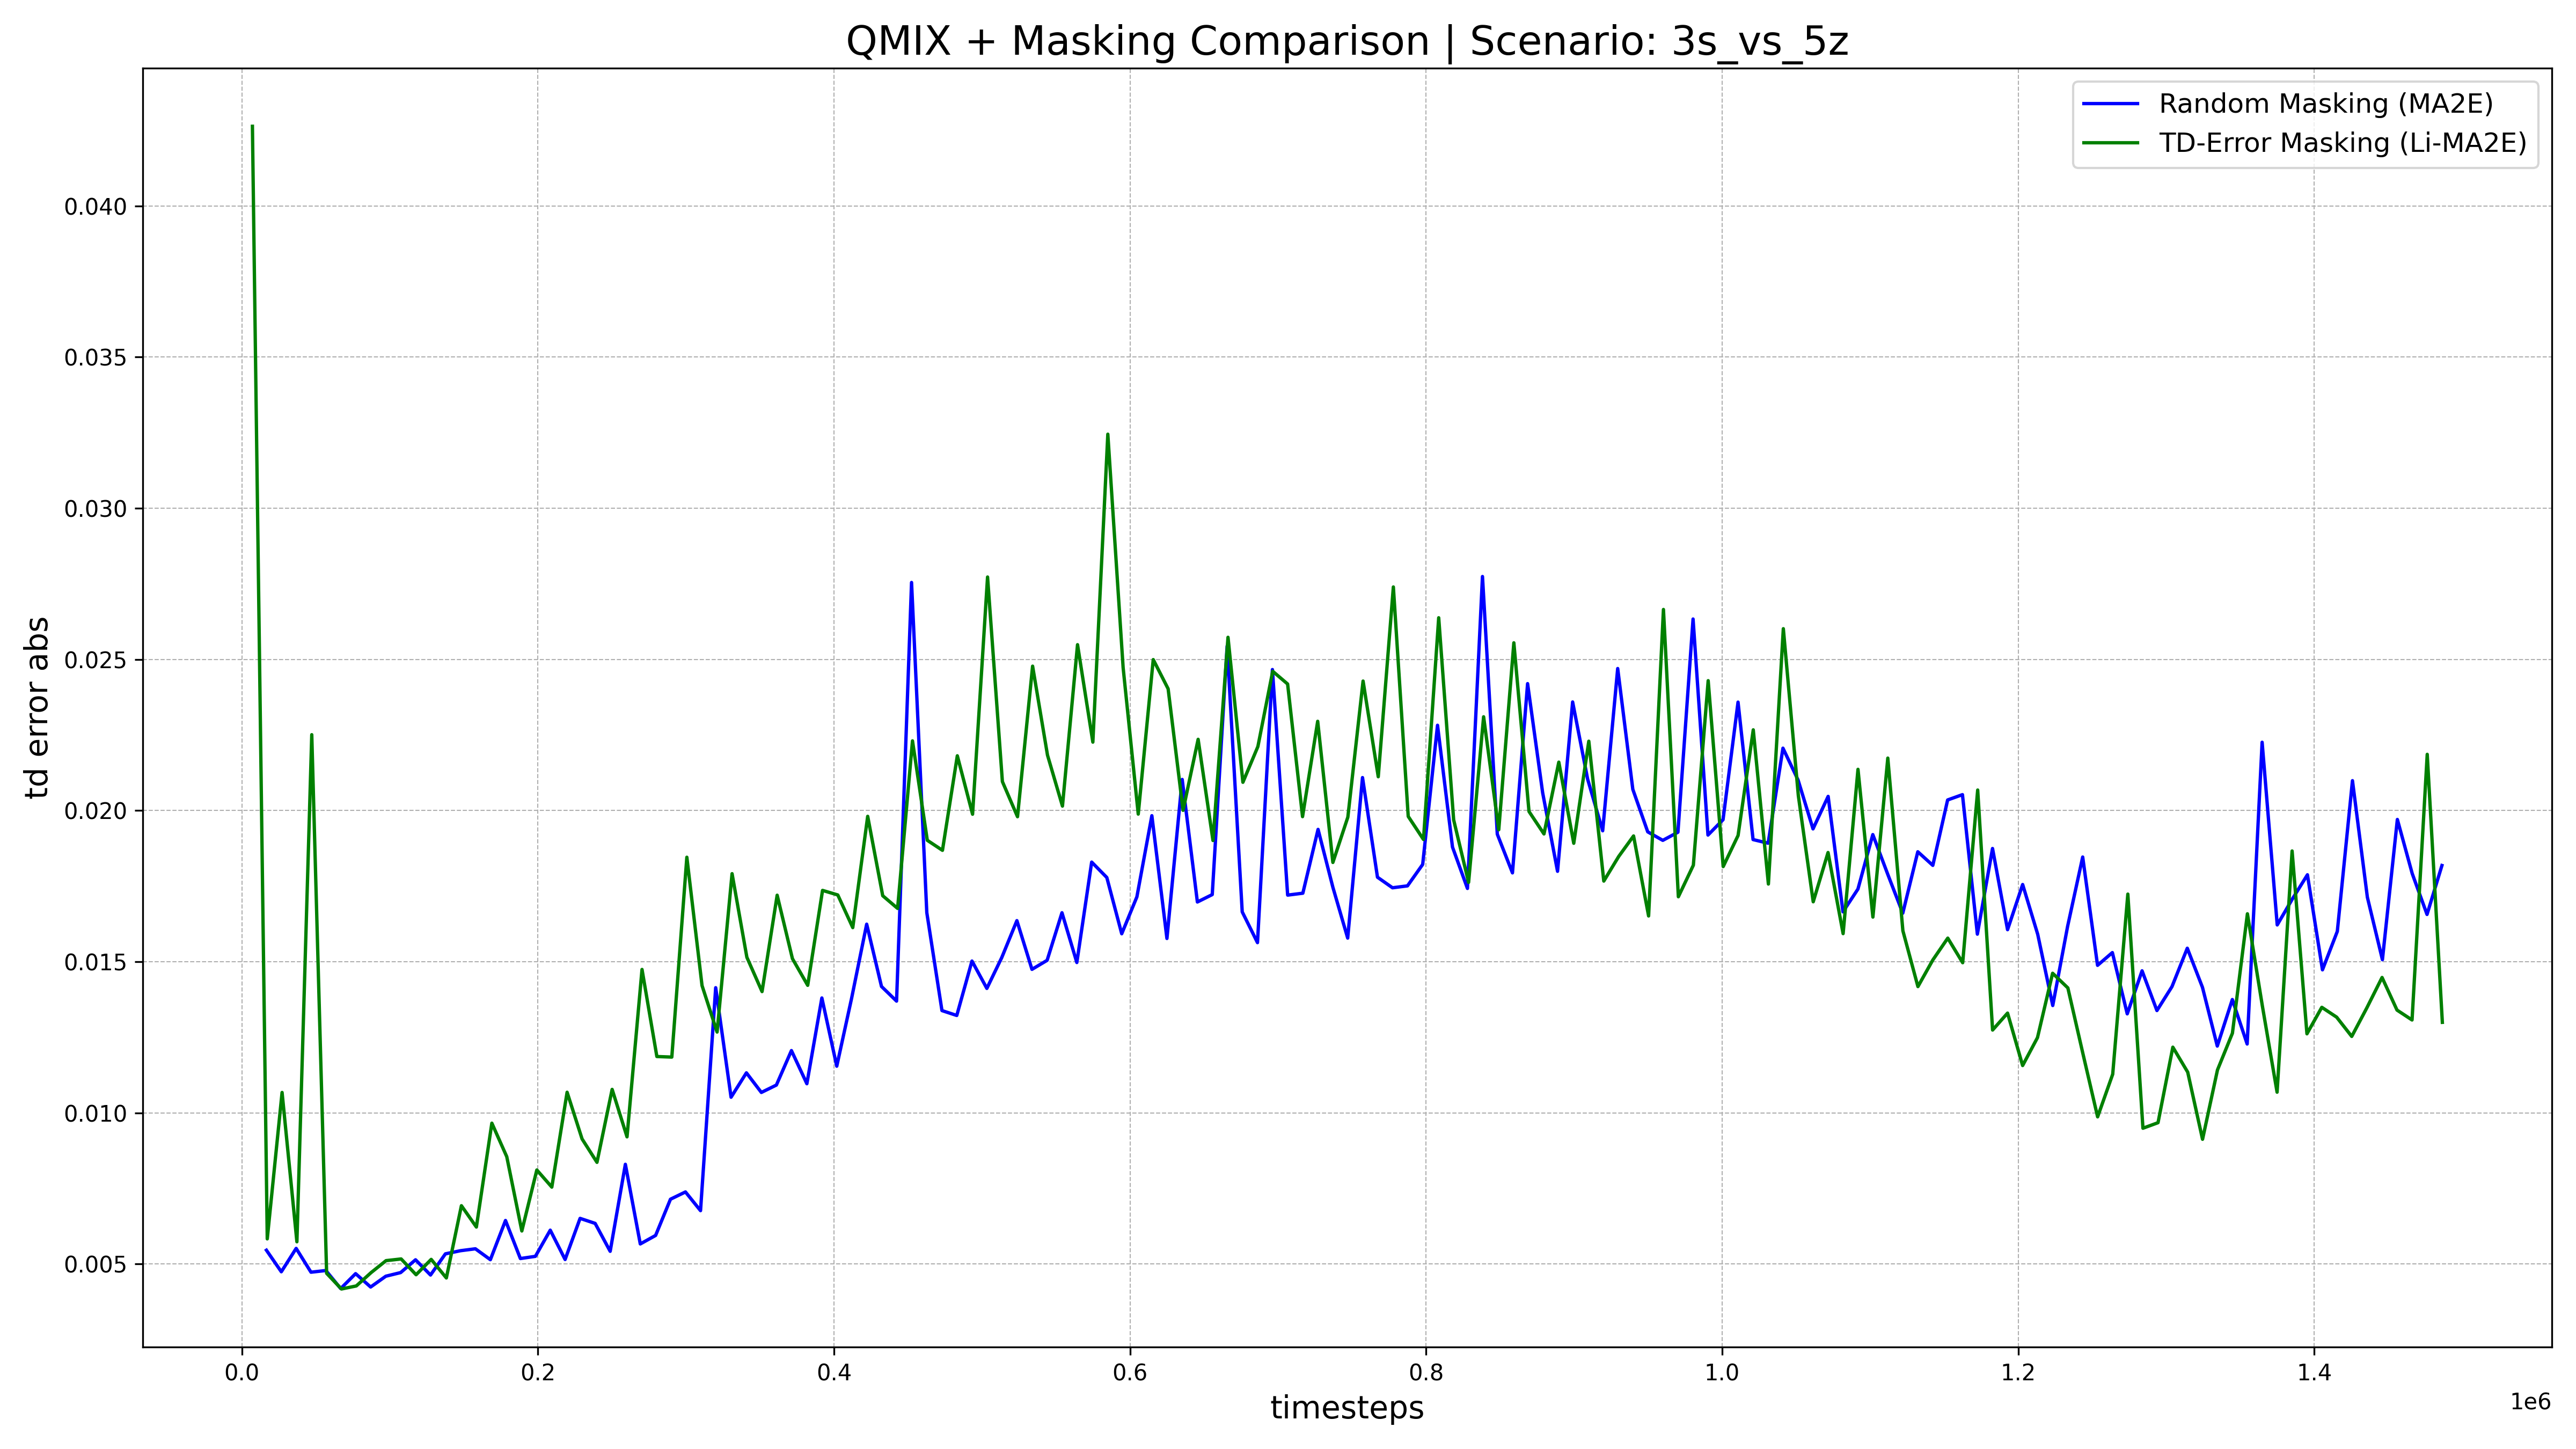
\includegraphics[width=0.32\textwidth]{images_pfe/results_td_error_abs/comparison_plot_3s_vs_5z.png}\label{fig:3s_vs_5z_td_error}}
    
    \caption{Mean absolute TD-error for LI-MA2E (green) vs. baseline Random Masking (blue) across various SMAC scenarios.}
    \label{fig:all_td_errors}
\end{figure}

\paragraph{Analysis}
The mean absolute TD-error plots in Figure~\ref{fig:all_td_errors} provide a clear and consistent insight into the learning dynamics of our $LI-MA^2E$ framework compared to the baseline. Across all scenarios, our intelligent masking strategy leads to a more stable and effective learning process. In the homogeneous maps \texttt{3m} and \texttt{8m}, the baseline method exhibits dramatic spikes in TD-error during training, indicating periods of high instability. Our $LI-MA^2E$ method, in contrast, maintains a consistently lower and more stable error, suggesting it helps prevent such instabilities. In more complex scenarios like \texttt{3s\_vs\_4z}  and \texttt{3s\_vs\_5z}, the baseline's TD-error remains stubbornly high for longer periods, whereas $LI-MA^2E$ is able to control and suppress the error much more effectively. This demonstrates that by actively focusing the MAE's reconstruction on agents with high prediction error, our framework creates a curriculum that directly and efficiently minimizes that error across the team. This more stable learning process is the underlying reason for the superior policy quality and performance gains detailed in the main results chapter.
% \chapter{Algorithms}

% \section*{Iterative Policy Evaluation Algorithm}
% \begin{algorithm}[H]
%     \caption{Iterative Policy Evaluation Algorithm}
%     \begin{algorithmic}[1]
%         \State Initialize $V(s) = 0$ for all $s \in \mathcal{S}$ (or arbitrarily)
%         \State $\theta > 0$ (a small threshold)
%         \State $\gamma$ (discount factor) where $0 \leq \gamma \leq 1 $
%         \Repeat
%             \State $\Delta \leftarrow 0$
%             \For{each state $s \in \mathcal{S}$}
%                 \State $v \leftarrow V(s)$
%                 \State $V(s) \leftarrow \sum_{a} \pi(a|s) \sum_{s', r} p(s', r|s, a) \left[ r + \gamma V(s') \right]$
%                 \State $\Delta \leftarrow \max(\Delta, |v - V(s)|)$
%             \EndFor
%         \Until{$\Delta < \theta$}
%     \end{algorithmic}
% \end{algorithm}



% \section*{Value Iteration Algorithm}
% \begin{algorithm}[H]
%     \caption{VALUE ITERATION}
%     \label{alg:value_iteration}
%     \begin{algorithmic}
%         \State \textbf{Initialize} \(V_0(s)\) arbitrarily (often set to 0 for all states)
        
%         \For{each iteration \(k\)}
      
%        \For{each state \(s \in \mathcal{S}\)}
           
%                 \State Update the value function \(V_{k+1}(s)\) using the Bellman equation:
%                 \[
%                 V_{k+1}(s) = \max_{a \in \mathcal{A}} \sum_{s' \in \mathcal{S}} P(s'|s, a) \left[ R(s, a, s') + \gamma V_k(s') \right]
%                 \]
%             \EndFor
            
%             \State Check for convergence: if the change in value function is smaller than a predefined threshold, stop
%         \EndFor
%     \end{algorithmic}
% \end{algorithm}




% \section*{Peer Evaluation based dual DQN Algorithm}

%     \begin{algorithm}[H]
%         Initialize replay memory, $[Q_a ^{A}]$, $[Q_a ^{M}]$, and the target with random parameters.
%         \\ 
%         for \ episode < max-ep do
%         \\
%         \hspace*{0.5cm} Make \ observations
%         \\
%         \hspace*{0.5cm} for \ t$<$time-steps:
%         \\
%         \hspace*{0.9cm} select\  action \ using \ $\epsilon - greedy$
%         \\
%         \hspace*{0.9cm} retrieve \ next observation \  and \  reward 
%         \\
%         \hspace*{0.9cm} calculate \  peer \ evaluation \  $z_a ^t$ \ for \  each \ agent \ $a$
%         \\
%         \hspace*{0.9cm} identify \ peers \ $K_a$ \ and \ aggregate \ the \ peer \ evaluations
%         \\
%         \hspace*{0.9cm} Store \ transition \ $(o^t, u^t, r^t, o^{t+1}, Z^t)$ \ in \ D
%         \\
%         \hspace*{0.9cm} \textbf{if} \ t$>$ warm-up-period \ \textbf{then:}
%         \\
%         \hspace*{1.2cm} $\hat{r} _a = r_a + \beta Z_a$ for each agent a 
%         \\
%         \hspace*{0.9cm} \textbf{end if}
%         \\ 
%         \hspace*{0.5cm} For each agent, update Neural Networks by minimizing the loss: 
%         \\
%         \hspace*{1.2cm} $L_a ^{A} (o_a, u_a, r_a, o'_a | \theta _a ^{A} , \theta _a ^{A'} = \sum ( Q^{A} (o,u | \theta _a ^{A} - y_a^{A} (o', r | \theta _a ^{A'}))^2$

%         \caption{Peer Evaluation based Dual DQN Training Algorithm}
%     \end{algorithm}



% \section*{Introspective Learning Algorithm}
% \begin{algorithm}[H]
%     \caption{INTROSPECTION LEARNING}
%     \label{alg:introspection_learning}
%     \begin{algorithmic}[1]
%         \State \textbf{Data:} Off-policy RL algorithm OPRL, policy function $\pi$, family of queries $(U_i)_i$, a schedule $\sigma$, a reward cutoff $R$
        
%         \State Initialize OPRL policy $\pi$ with random weights $\vartheta$ and replay buffer $D$
        
%         \For{episode $e \in \{1, \ldots, M\}$}
        
%         \hspace*{0.4cm}    \State Train OPRL as specified
            
%            \hspace*{0.4cm} \If{moving average reward $< R$ and $e \in \sigma$}
            
%               \hspace*{1cm} For each $i$
%                  query $\omega_\pi (U_i)$ and add examples $\omega _\pi (U_i) \in S$ to $D$ as terminal
%             \EndIf
%         \EndFor
%     \end{algorithmic}
% \end{algorithm}






% \clearpage

% \section*{Learning from Demonstration Algorithm}

% \begin{algorithm}
% \caption{Introspective Q-Learning}
% \begin{algorithmic}


% \textbf{Require:} discount factor $\gamma$, learning rate $\alpha$, queue size $qs$

% \textbf{Procedure:} {Introspective Q-Learning}{}

%     \hspace*{0.4cm} \State initialise value-function $Q$ to all 0.
    
%    \hspace*{0.4cm}   \State initialise the priority queue $PQ$ (empty or with demonstrations)
    
%     \hspace*{0.4cm}  \For{each step of episode}
    
%        \hspace*{0.8cm}   \State $s_t$ is initialised as the starting state
        
%         \hspace*{0.8cm} \State choose $a_t$ in $s_t$ using $\pi$ derived from $Q$
        
%     \hspace*{0.8cm}     \State $SC \gets$ empty list
%         \Comment $SC$ collects all experience tuples $(s, a, s', r)$ in an episode
        
%      \hspace*{0.8cm}   \textbf{Repeat}
        
%         \hspace*{1.2cm}    \State perform action $a_t$
            
%          \hspace*{1.2cm}    \State observe reward $r_t$ and new state $s_{t+1}$
            
%           \hspace*{1.2cm}   \State choose $a_{t+1}$ in $s_{t+1}$ using $\pi$ derived from $Q$
            
%           \hspace*{1.7cm}   \State $Q(s_t, a_t) \gets Q(s_t, a_t) $
          
%        \hspace*{1.7cm}   \State   $ + \alpha \big(r_t + F(s_t, a_t, s_{t+1}, a_{t+1})$
       
%        \hspace*{1.7cm}   \State 
%       $ + \gamma \max\limits_b Q(s_{t+1}, b) - Q(s_t, a_t)\big)$
            
%          \hspace*{1.2cm}   \State insert $(s_t, a_t, s_{t+1}, r_t)$ to $SC$
%             \Comment Collect steps
            
%          \hspace*{1.2cm}   \State $s_t \gets s_{t+1}$
            
%          \hspace*{1.2cm}   \State $a_t \gets a_{t+1}$
            
%         \hspace*{0.8cm}  \textbf{Until} $s_t$ is a terminal state
        
%        \hspace*{0.8cm}   \For{each $(s_t, a_t, s_{t+1}, r_t)$ in $SC$}
        
%         \hspace*{1.2cm}   \For{$i$ in $[0, 1, \ldots, \text{length}(SC) - t]$}
        
%           \hspace*{1.7cm}  \State $q_{bt} \gets q_{bt} + \gamma^i r_{t+i}$
        
%         \hspace*{1.2cm}   \State Filter($\langle s_t, a_t, q_{bt} \rangle$, $PQ$)
%         \EndFor
%     \EndFor
% \EndProcedure

% \end{algorithmic}
% \end{algorithm}









\newpage

\chapter{Benchmark Environment Specifications}
\section{SMAC Environment Details}


\begin{table}[H]
\centering

% --- CUSTOMIZATION CONTROLS ---

% 1. Use a smaller font if needed (\small, \footnotesize, or \scriptsize)
\small 

% 2. Reduce horizontal space between columns (default is 6pt)
\setlength{\tabcolsep}{4pt}

% 3. Reduce vertical padding between rows (1.0 is standard, <1.0 is tight)
\renewcommand{\arraystretch}{1.1} 

% --- TABLE DEFINITION ---

% We define specific widths for columns 2, 3, and 4 to control wrapping.
% The 'c' centers the first column. The '>{\centering\arraybackslash}' part
% makes the text inside the paragraph columns centered.
\begin{tabular}{c >{\centering\arraybackslash}p{3cm} >{\centering\arraybackslash}p{3cm} >{\centering\arraybackslash}p{2.5cm}} 
\hline
\textbf{Name} & \textbf{Ally Units} & \textbf{Enemy Units} & \textbf{Type} \\
\hline
3m & 3 Marines & 3 Marines & homogeneous \& symmetric \\
\hline
8m & 8 Marines & 8 Marines & homogeneous \& symmetric \\
\hline
25m & 25 Marines & 25 Marines & homogeneous \& symmetric \\
\hline
2s3z & 2 Stalkers \& 3 Zealots & 2 Stalkers \& 3 Zealots & heterogeneous \& symmetric \\
\hline
3s5z & 3 Stalkers \& 5 Zealots & 3 Stalkers \& 5 Zealots & heterogeneous \& symmetric \\
\hline
MMM & 1 Medivac, 2 Marauders \& 7 Marines & 1 Medivac, 2 Marauders \& 7 Marines & heterogeneous \& symmetric \\
\hline
5m\_vs\_6m & 5 Marines & 6 Marines & homogeneous \& asymmetric \\
\hline
8m\_vs\_9m & 8 Marines & 9 Marines & homogeneous \& asymmetric \\
\hline
10m\_vs\_11m & 10 Marines & 11 Marines & homogeneous \& asymmetric \\
\hline
27m\_vs\_30m & 27 Marines & 30 Marines & homogeneous \& asymmetric \\
\hline
3s5z\_vs\_3s6z & 3 Stalkers \& 5 Zealots & 3 Stalkers \& 6 Zealots & heterogeneous \& asymmetric \\
\hline
MMM2 & 1 Medivac, 2 Marauders \& 7 Marines & 1 Medivac, 3 Marauders \& 8 Marines & heterogeneous \& asymmetric \\
\hline
2m\_vs\_1z & 2 Marines & 1 Zealot & micro-trick: alternating fire \\
\hline
\end{tabular}

\caption{SMAC Map Scenarios (Part 1).}
\label{tab:smac_senarios_part1}
\end{table}

\begin{table}[H]
\centering

% --- CUSTOMIZATION CONTROLS ---

% 1. Use a smaller font if needed (\small, \footnotesize, or \scriptsize)
\small 

% 2. Reduce horizontal space between columns (default is 6pt)
\setlength{\tabcolsep}{4pt}

% 3. Reduce vertical padding between rows (1.0 is standard, <1.0 is tight)
\renewcommand{\arraystretch}{1.1} 

% --- TABLE DEFINITION ---

% We define specific widths for columns 2, 3, and 4 to control wrapping.
% The 'c' centers the first column. The '>{\centering\arraybackslash}' part
% makes the text inside the paragraph columns centered.
\begin{tabular}{c >{\centering\arraybackslash}p{3cm} >{\centering\arraybackslash}p{3cm} >{\centering\arraybackslash}p{2.5cm}} 
\hline
\textbf{Name} & \textbf{Ally Units} & \textbf{Enemy Units} & \textbf{Type} \\
\hline
2s\_vs\_1sc & 2 Stalkers & 1 Spine Crawler & micro-trick: alternating fire \\
\hline

3s\_vs\_3z & 3 Stalkers & 3 Zealots & micro-trick: kiting \\
\hline
3s\_vs\_4z & 3 Stalkers & 4 Zealots & micro-trick: kiting \\
\hline
3s\_vs\_5z & 3 Stalkers & 5 Zealots & micro-trick: kiting \\
\hline
6h\_vs\_8z & 6 Hydralisks & 8 Zealots & micro-trick: focus fire \\
\hline
corridor & 6 Zealots & 24 Zerglings & micro-trick: wall off \\
\hline
bane\_vs\_bane & 20 Zerglings \& 4 Banelings & 20 Zerglings \& 4 Banelings & micro-trick: positioning \\
\hline
so\_many\_banelings & 7 Zealots & 32 Banelings & micro-trick: positioning \\
\hline
2c\_vs\_64zg & 2 Colossi & 64 Zerglings & micro-trick: positioning \\
\hline
1c3s5z & 1 Colossi \& 3 Stalkers \& 5 Zealots & 1 Colossi \& 3 Stalkers \& 5 Zealots & heterogeneous \& symmetric \\
\hline
\end{tabular}
\caption{SMAC Map Scenarios (Part 2).}
\label{tab:smac_senarios_part2}
\end{table}